% Options for packages loaded elsewhere
\PassOptionsToPackage{unicode}{hyperref}
\PassOptionsToPackage{hyphens}{url}
\documentclass[
  10pt,
]{article}
\usepackage{xcolor}
\usepackage[margin=0.75in,letterpaper]{geometry}
\usepackage{amsmath,amssymb}
\setcounter{secnumdepth}{-\maxdimen} % remove section numbering
\usepackage{iftex}
\ifPDFTeX
  \usepackage[T1]{fontenc}
  \usepackage[utf8]{inputenc}
  \usepackage{textcomp} % provide euro and other symbols
\else % if luatex or xetex
  \usepackage{unicode-math} % this also loads fontspec
  \defaultfontfeatures{Scale=MatchLowercase}
  \defaultfontfeatures[\rmfamily]{Ligatures=TeX,Scale=1}
\fi
\usepackage{lmodern}
\ifPDFTeX\else
  % xetex/luatex font selection
\fi
% Use upquote if available, for straight quotes in verbatim environments
\IfFileExists{upquote.sty}{\usepackage{upquote}}{}
\IfFileExists{microtype.sty}{% use microtype if available
  \usepackage[]{microtype}
  \UseMicrotypeSet[protrusion]{basicmath} % disable protrusion for tt fonts
}{}
\makeatletter
\@ifundefined{KOMAClassName}{% if non-KOMA class
  \IfFileExists{parskip.sty}{%
    \usepackage{parskip}
  }{% else
    \setlength{\parindent}{0pt}
    \setlength{\parskip}{6pt plus 2pt minus 1pt}}
}{% if KOMA class
  \KOMAoptions{parskip=half}}
\makeatother
\usepackage{longtable,booktabs,array}
\usepackage{caption}
\newcounter{none} % for unnumbered tables
\usepackage{calc} % for calculating minipage widths
% Correct order of tables after \paragraph or \subparagraph
\usepackage{etoolbox}
\makeatletter
\patchcmd\longtable{\par}{\if@noskipsec\mbox{}\fi\par}{}{}
\makeatother
\usepackage{graphicx}
\makeatletter
\newsavebox\pandoc@box
\newcommand*\pandocbounded[1]{% scales image to fit in text height/width
  \sbox\pandoc@box{#1}%
  \Gscale@div\@tempa{\textheight}{\dimexpr\ht\pandoc@box+\dp\pandoc@box\relax}%
  \Gscale@div\@tempb{\linewidth}{\wd\pandoc@box}%
  \ifdim\@tempb\p@<\@tempa\p@\let\@tempa\@tempb\fi% select the smaller of both
  \ifdim\@tempa\p@<\p@\scalebox{\@tempa}{\usebox\pandoc@box}%
  \else\usebox{\pandoc@box}%
  \fi%
}
% Set default figure placement to htbp
\def\fps@figure{htbp}
\makeatother
\setlength{\emergencystretch}{3em} % prevent overfull lines
\providecommand{\tightlist}{%
  \setlength{\itemsep}{0pt}\setlength{\parskip}{0pt}}
% header.tex -- build-only preamble for the seam manuscript draft.
% Not part of the manuscript; passed with --include-in-header.
% Assumes the Pandoc XeLaTeX template has already loaded fontspec,
% unicode-math, longtable, booktabs, array, caption, calc, etoolbox.

% ---------------------------------------------------------------------
% 1. Unicode text-mode glyphs that Latin Modern Roman does not carry.
%    Each is mapped to the equivalent math macro, so it typesets from
%    Latin Modern Math and stays searchable/copyable in the PDF only
%    where the source glyph survives (math macros are not ToUnicode).
%    U+2605 (★) has no Latin Modern Math glyph, so it maps to the
%    Latin Modern Math star operator U+22C6 (\star) rather than pulling
%    in a platform symbol font. No Segoe UI Symbol fallback remains.
% ---------------------------------------------------------------------
\usepackage{newunicodechar}
% unicode-math installs its own begin-document definitions for math
% characters, so the mappings must be declared inside \AtBeginDocument
% to run after them; a plain preamble \newunicodechar is overwritten.
\AtBeginDocument{%
  \newunicodechar{★}{\ensuremath{\star}}%
  \newunicodechar{⊆}{\ensuremath{\subseteq}}%
  \newunicodechar{→}{\ensuremath{\rightarrow}}%
  \newunicodechar{ρ}{\ensuremath{\rho}}%
  \newunicodechar{τ}{\ensuremath{\tau}}%
  \newunicodechar{≔}{\ensuremath{\mathrel{:=}}}%
  \newunicodechar{⊓}{\ensuremath{\sqcap}}%
  \newunicodechar{∧}{\ensuremath{\wedge}}%
  \newunicodechar{∈}{\ensuremath{\in}}%
  \newunicodechar{≡}{\ensuremath{\equiv}}%
  \newunicodechar{′}{\ensuremath{{}^{\prime}}}%
}

% ---------------------------------------------------------------------
% 2. Captions. The manuscript writes its own "**Figure 1.**" label in
%    the caption text, so suppress LaTeX's "Figure 1:" prefix to avoid
%    a duplicated label. Table captions are ordinary body paragraphs
%    (Pandoc pipe tables carry no \caption), so this only affects figures.
% ---------------------------------------------------------------------
\captionsetup{labelformat=empty,justification=raggedright,singlelinecheck=false,font=small}

% ---------------------------------------------------------------------
% 3. Tables. Sixteen pipe tables become sixteen longtables. Long arm
%    names in \texttt cannot hyphenate, so widen the usable measure by
%    shrinking table type and inter-column padding.
% ---------------------------------------------------------------------
\AtBeginEnvironment{longtable}{\footnotesize}
\setlength{\tabcolsep}{3pt}
\renewcommand{\arraystretch}{1.12}
\setlength{\LTpre}{6pt}
\setlength{\LTpost}{6pt}

% ---------------------------------------------------------------------
% 4. Floats: keep figures near their references in a single-column draft.
% ---------------------------------------------------------------------
\usepackage{float}
\floatplacement{figure}{htbp}
\renewcommand{\topfraction}{0.92}
\renewcommand{\bottomfraction}{0.8}
\renewcommand{\textfraction}{0.08}
\renewcommand{\floatpagefraction}{0.75}

% ---------------------------------------------------------------------
% 5. Author block. Pandoc escapes backslashes in YAML author metadata,
%    so set the multi-line display form after the template has run.
% ---------------------------------------------------------------------
\AtBeginDocument{%
  \author{Prathamesh Patil\\Department of Computer Engineering\\Sardar Patel Institute of Technology}%
  \hypersetup{pdfauthor={Prathamesh Patil}}%
}

% --- variant B: long code spans are wrapped selectively by the build
%     post-process, not globally; global seqsplit breaks status tokens
%     such as SUPPORTED mid-word.
\usepackage{seqsplit}
\usepackage{url}
\usepackage{needspace}
\let\origtexttt\texttt
% Inline code and artifact paths stay upright even inside italic notes.
% \upshape changes only the shape, so bold table/heading contexts keep their
% weight.  The url package's \path command selects \UrlFont directly, so it
% needs the same rule.
\renewcommand{\texttt}[1]{{\upshape\origtexttt{#1}}}
\makeatletter
\def\url@ttstyle{\def\UrlFont{\ttfamily\upshape}}
\makeatother
\setlength{\emergencystretch}{4em}
% Overfull boxes are counted from the log; do not print debug rules in the
% candidate PDF (they read as black artifacts in narrow table columns).
\overfullrule=0pt

% --- variant C: allow a break after escaped underscores in plain text
\let\origunderscore\_
\renewcommand{\_}{\origunderscore\allowbreak}

% --- variant F: inside longtables, use the original \texttt so cells
%     break only at separators, not mid-token.
\AtBeginEnvironment{longtable}{\let\texttt\origtexttt}

\usepackage{bookmark}
\IfFileExists{xurl.sty}{\usepackage{xurl}}{} % add URL line breaks if available
\urlstyle{same}
% fallback for those not using the hyperref driver hyperxmp:
\makeatletter
\@ifundefined{xmpquote}{\newcommand{\xmpquote}[1]{#1}}{}
\makeatother
\hypersetup{
  pdftitle={The Handoff Nobody Owns: Measuring What Cross-Mechanism Authorization Seams Cannot Carry},
  pdfauthor={Prathamesh Patil},
  pdfkeywords={\xmpquote{cross-mechanism authorization; agent
authorization; authorization seams; scope narrowing; evidence carriage;
conformance testing; locked-artifact methodology}},
  hidelinks,
  pdfcreator={LaTeX via pandoc}}

\title{The Handoff Nobody Owns: Measuring What Cross-Mechanism
Authorization Seams Cannot Carry}
\author{Prathamesh Patil}
\date{26 October 2026}

\begin{document}
\maketitle

\begin{abstract}

Agent authorization rarely stops at a mechanism boundary. A sender
narrows its authority, a bridge translates the narrowed decision into a
record the receiver can read, and the receiver applies its own admission
rules. Each component can behave correctly in isolation while the
composed system admits a call the sender never authorized. This paper
studies that cross-mechanism handoff as a measurement problem. We
describe a locked-artifact method: predictions, cases, arms, and hashes
are frozen before execution; runs are sequential, offline, and
deterministic; discrepancies are reconciled verbatim; and reported
values are generated from stored artifacts rather than transcribed by
hand. Across the mechanism pairs, the action-narrowing extension, and
the boundary study of bridge variants, we test whether composition adds
authorization failures beyond those a receiving mechanism already
exhibits standalone. On the frozen case families, the answer is scoped:
under narrowing-preserving bridge mappings, composition adds no
admission beyond the receiver's own, with a measured exception in an
action-narrowing family whose attribution depends on the scoring
convention. The exception is bounded to its design point and case
family. We distinguish receiver-side and bridge-side repair loci:
consumption or evidence carriage when the narrowed fact crosses intact,
and derivation repair when the bridge itself widens authority. We close
with the conformance kit prepared for others to run these seam tests
against their own bridge and mechanism pairs.

\textbf{Keywords:} cross-mechanism authorization; agent authorization;
authorization seams; scope narrowing; evidence carriage; conformance
testing; locked-artifact methodology

\end{abstract}

\section{1. Introduction}\label{introduction}

At every cross-mechanism handoff in agent authorization, three parties
meet at a seam that nobody owns. The sender holds authority A over a
call space C and narrows that authority to A′ ⊆ A before sending the
call onward. The bridge translates the sender's narrowed decision and
state into a receiver-side record \mbox{ρ\_R} = B(A′, state). The receiver,
running its own mechanism M\_R = (V\_R, admit\_R), decides whether to
admit the call. Each party can be faithful inside its own world: the
sender's narrowing can be exact, the bridge's transport can be
byte-perfect, and the receiver's verdict can still be an admission the
sender never authorized. The gap is not that the record is unfaithful;
it is that a faithful scope record cannot carry, and the receiver cannot
derive, an authorization decision. A call can cross the seam on a
byte-perfect record while the authority behind it does not cross with
it. That is the handoff problem this section locates: no single
mechanism owns the seam, and the seam carries less context than the
receiver's checks would need to detect standing authority violations on
their own.

Why a faithful record is not enough is the formal core's blindness
point, introduced here as a decision rule rather than as a measured
result: ``carried but unread = uncarried (for decision purposes).'' The
receiver's read set V\_read ⊆ V\_R is the set of fields the decision
actually consults --- not what the record carries, but what the decision
reads. A fact in the carried record that no decision reads constrains no
decision, even when the transport was byte-perfect. The narrowed action
can cross intact and the synthesis can simply never consume it. Measured
instances of this blindness appear in Sections 4--5; in this section the
aphorism does the work of the formal core's decision rule, and nothing
in this section is presented as a measurement.

The research question follows directly: at a cross-mechanism handoff,
does the composed system enforce the sender's narrowing, or does the
seam admit calls the narrowing never conferred?

Conditional answer preview: under narrowing-preserving mappings
(canonical T0) on the frozen case sets, the seam test shows zero seam
--- composition creates no authorization failure that one of the
mechanisms does not already exhibit standalone --- with one measured,
convention-scoped exception (the E1 action family under arm-native
scoring) that is disclosed and bounded where it is reported later, not
claimed as a universal here. The zero is a recorded property of
narrowing-preserving mappings on these case sets, not a theorem: as
operationalized, the seam test can fire only where the composition
widens, and the single measured composition-specific exception is the E1
action family under arm-native scoring, where it does. This is the
bounded zero-seam finding, ★ \texttt{SUPPORTED}: zero seam is a property
of narrowing-preserving mappings on the frozen case sets, bounded rather
than assumed, and it holds only with its three conditions named together
--- narrowing-preserving mappings (canonical T0), frozen case sets, and
disclosure of the exception and bridge artifacts. Where a bridge is not
narrowing-preserving, the seam can leak with or without composition;
that fault belongs to the bridge's manifest derivation rather than to
composition itself, and it is disclosed here only as a condition,
without numbers. Zero seam is therefore not universal in either
direction: it does not assert seam safety, and it does not assert
general seam failure. The star (★) marks the frozen cross-cutting claim,
not a significance test. The zero is also partly construction-forced: in
Pilot 1 and the SentinelAgent pair, the composed arm and the standalone
receiving arm share the same contract and scoring, so their leak sets
are identical by construction and carry no evidential weight about
composition. E1 is the only genuine composition-specific test in this
program; it is one design point × four attack cases and is
convention-dependent. The zero is therefore a bounded design property,
not an empirical discovery that composition cannot add authority.

\textbf{Hypothesis key.} H1 --- trusted-request laundering / scope
trust; H2 --- dynamic state, identity, and freshness do not cross and
leak; H3 --- state/identity vocabulary gaps manifest as silence, not
misparse; H4 --- no shared audit trail (\texttt{UNTESTED}); H5 ---
verification attests key possession and integrity, not authority; H6 ---
similar-pair vs dissimilar-pair failure shapes; H7 --- intent layer P2
(\texttt{UNTESTED}); ★ --- the cross-cutting zero-under-preservation
finding. The frozen experiment artifacts predate this key and use some
labels differently; Appendix Table A1 records the lineage, and a legacy
label is not read as the current label with the same number.

Scope-trust framing, carried as H1 \texttt{REFINED}: at a
cross-mechanism handoff the receiving mechanism re-derives scope, or
trusts the already-authorized caller, in a way that can admit a call the
upstream narrowing did not confer. The gap is not that the record is
unfaithful but that a faithful scope record cannot carry, and the
receiver cannot derive, an authorization decision. Scope trust matters
precisely because the receiver's re-derivation can differ from the
sender's intent: a call admitted inside the receiver's own vocabulary
may never have been authorized at the sender at all. The resource clause
of this framing is not supported. The action clause is measured under
M0; its composition-specific attribution is read under arm-native
scoring. H1 is refined, not settled: the action clause is measured under
M0, with the composition-specific attribution under arm-native scoring;
the resource clause is not supported; and the framing is extended to the
bridge's manifest derivation where that derivation widens scope. Nothing
here upgrades either clause into a universal claim about scope
laundering across arbitrary bridges.

Key-distribution preview, carried as H5 \texttt{REFINED}: a validly
signed token attests to integrity and key possession, not the source of
authority --- scoped to the SentinelAgent pair; key distribution is the
critical interface at the seam. A receiver that verifies a signature
learns key possession and payload integrity; it does not learn who
minted the record, and any keyholder is, to that receiver, equivalent to
the issuer within the token vocabulary. Verification therefore attests
to the token's intactness and to possession of the signing key, while
the question of authority --- who is entitled to act --- must be settled
elsewhere, at the key-distribution interface. That preview is scoped to
the SentinelAgent pair and to the frozen prototype's key model; nothing
here extends it to other key models or to live attestation services, and
nothing here says that signed evidence is unsafe or that verification
itself is the flaw.

Disclosures: conditional language only --- nothing in this section is an
unconditioned universal. The seam is not asserted safe by default, and
no claim about seam safety in either direction is made without its
conditions. Nothing here asserts priority over prior work, and nothing
is framed as a new contribution beyond the frozen positioning. Every
positive sentence in this section stays conditional: the zero-seam
result, the scope-trust framing, and the key-distribution preview all
carry their conditions in the same passage. Figure 1 presents this
anatomy as a schematic.

\begin{figure}
\centering
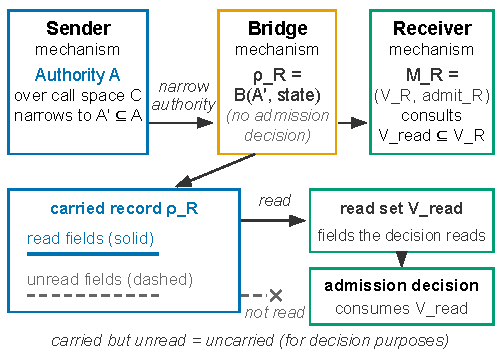
\includegraphics[width=3.33in,height=\textheight,keepaspectratio,alt={Figure
1. Anatomy of a cross-mechanism handoff --- the sender narrows
authority, the bridge translates it into a receiver-side record, and the
receiver decides; the schematic distinguishes the record the bridge
carries from the read set the receiver's decision actually
consults.}]{figures/figure_1_handoff_anatomy.pdf}
\caption{\textbf{Figure 1.} Anatomy of a cross-mechanism handoff --- the
sender narrows authority, the bridge translates it into a receiver-side
record, and the receiver decides; the schematic distinguishes the record
the bridge carries from the read set the receiver's decision actually
consults.}\label{fig:figure1}
\end{figure}

The schematic carries no data and no numbers, and no labels beyond those
defined here.

Sender: call c ∈ C; authority A ⊆ C; narrows A → A′. Bridge (the seam)
B: \mbox{ρ\_R} = B(A′, state) --- the receiver-side record built from the
narrowed decision plus state. Receiver: mechanism M\_R = (V\_R,
admit\_R); read set V\_read ⊆ V\_R --- the fields the decision consults,
not what the record carries. Composition: admit\_C(c) ≔ admit\_R(c,
B(A′)); effective authority A\_C ≔ \{ c: admit\_C(c) = allow \}.

A fact in the carried record that no decision reads constrains no
decision --- that is the blindness the formal core names, and it is why
the seam can admit what the sender never narrowed. Sender, bridge, and
receiver each discharge their own duties, and no mechanism is assigned
responsibility for the seam between them.

\section{2. Background --- APC (Agentic Principal Chain), TraceGrant,
SentinelAgent; Progent as
reference}\label{background-apc-agentic-principal-chain-tracegrant-sentinelagent-progent-as-reference}

This section places the three formal spines whose within-mechanism
guarantees leave the cross-mechanism slot uncovered, and it reports each
upstream guarantee as its authors' self-report --- never upgraded to a
manuscript result and never cited as this program's measurement. None of
the three spines supplies a cross-mechanism composition guarantee; the
observation is scoped to these three systems and is not a universal
negative. The purpose is to show where each guarantee stops, so that the
uncovered slot --- the seam between mechanisms --- can be named plainly.

APC {[}APC{]} --- the Agentic Principal Chain mechanism --- reports
within-mechanism authorization: a scope algebra with meet ⊓, conditions
C1--C6, and Thm 4.7 (Composition Soundness), conditional on a complete
effective restriction set, serialized admission, and a static X within a
session. APC's ``composition'' is composition of action sequences inside
one session; it is not composition across mechanisms. Its resource meet
holds inside the mechanism. APC alone governs calls inside one
mechanism; it says nothing about what happens when a narrowed call
crosses into another mechanism's vocabulary, and it supplies no
cross-mechanism composition guarantee. Its authorization reasoning is
sound only relative to the assumptions the theorem names, and nothing in
APC extends that reasoning across a bridge to a receiver with a
different vocabulary.

TraceGrant {[}TraceGrant{]} reports within-mechanism delegation: POEC
contracts, Eq. 2 / Algorithm 1. Its soundness is assumed (Eq. 10 is not
proven). Like APC, TraceGrant's guarantee stays inside its own mechanism
and extends no composition claim across a seam. Delegation soundness is
an assumption of the formalism, not a result this program verifies, and
it covers calls handled within TraceGrant's own contract model rather
than calls handed off to another mechanism.

SentinelAgent {[}SentinelAgent{]} reports a token model τ with
principles P1--P7 (P1 and P3--P7 TLA+-checked; P2 probabilistic), a TLA+
model of 2.7M states --- an upstream self-report, not a measurement of
this program --- and Thm 4 (Composition Safety with Write-Impact
Notification), which is stated for two delegation chains that both
satisfy P1--P7 within its own framework. It does not state a guarantee
for a chain handed to a different mechanism's decision procedure; that
boundary is where this paper's cross-mechanism question begins. That
figure is the authors' own model-scale claim; this program neither
measured it nor relies on it as evidence.

The uncovered slot: within-mechanism guarantees do not compose across
mechanisms. None of APC, TraceGrant, or SentinelAgent supplies a
cross-mechanism composition guarantee. Scoped to these three --- no
universal negative --- the slot remains: what happens at the seam
between a sender's narrowing and a receiver's decision when the two
mechanisms do not share a vocabulary or a decision rule. The three
scopes differ in their limits, but they share the same boundary. APC's
theorem is conditional on a static X and governs intra-session
action-sequence composition inside one mechanism, so it says nothing
about a call crossing into another mechanism's vocabulary. TraceGrant's
soundness is assumed rather than proven (Eq. 10), so its delegation
guarantee covers contracts handled within TraceGrant's own model, not
calls handed off to another mechanism. SentinelAgent's theorem addresses
composition of two chains within its own P1--P7 framework, not a chain
handed to a different mechanism's decision procedure, so the
cross-mechanism case falls outside it. Each guarantee stops at its
mechanism's edge: a record can be faithful at the bridge and still carry
nothing the receiver's decision reads; a signature can be valid and
still attest nothing about the source of authority; a theorem
conditioned on a static state says nothing about a dynamic handoff.

This paper's position occupies that slot: narrowing-preservation plus
the blindness lemma --- cross-mechanism composition --- the slot the
others leave uncovered. The blindness lemma says a fact carried but
never read constrains no decision; narrowing-preservation requires the
composed system to enforce at least the sender's narrowing on the
relevant family. Together they name the guarantee the three spines leave
to the seam, and this program measures whether it holds on the frozen
case sets. The claim is deliberately scoped: it concerns these three
spines, these mappings, and these case sets, and it is not a universal
statement about every bridge or every mechanism pair.

Progent {[}Progent{]} is a close reference point rather than an input to
this program: it enforces monotonic confinement inside a single
privilege-control layer, where an SMT solver classifies each policy
update as a narrowing or an expansion; this paper asks whether a
comparable narrowing survives translation across a mechanism boundary.
Its reported results remain its authors' self-report and are not used as
an input or comparison here. Nothing about Progent is claimed or
measured in this section, and its results play no role in the paper's
measured claims.

Disclosures: say ``reports,'' never upgrade a self-report to an
established result; upstream guarantees and numbers stay self-reported;
nothing in this section impugns any upstream mechanism; no
production-safety claim; no benchmark comparability; citations are
pointers, not verified inputs. Citation keys are bracketed ---
{[}APC{]}, {[}TraceGrant{]}, {[}SentinelAgent{]}, {[}Progent{]} --- and
no bibliographic detail is invented. The industry/standards citation
layer belongs to Section 6 and is not invoked here. Table 1 summarizes
each formal spine and the scope of its composition claim.

\textbf{Table 1.} Formal spine and composition-claim scope.

{\def\LTcaptype{none} % do not increment counter
\begin{longtable}[]{@{}
  >{\raggedright\arraybackslash}p{(\linewidth - 4\tabcolsep) * \real{0.3333}}
  >{\raggedright\arraybackslash}p{(\linewidth - 4\tabcolsep) * \real{0.3333}}
  >{\raggedright\arraybackslash}p{(\linewidth - 4\tabcolsep) * \real{0.3333}}@{}}
\toprule\noalign{}
\begin{minipage}[b]{\linewidth}\raggedright
System
\end{minipage} & \begin{minipage}[b]{\linewidth}\raggedright
Formal spine
\end{minipage} & \begin{minipage}[b]{\linewidth}\raggedright
Composition-claim scope
\end{minipage} \\
\midrule\noalign{}
\endhead
\bottomrule\noalign{}
\endlastfoot
APC & scope algebra, meet ⊓, conditions C1--C6, Thm 4.7 (Composition
Soundness) & within APC, intra-session; conditional on complete
restriction set, serialized admission, static X \\
TraceGrant & POEC contracts, Eq. 2 / Algorithm 1 & soundness assumed
(Eq. 10), not proven \\
SentinelAgent & token τ, P1--P7, TLA+ (2.7M states), Thm 4 (Composition
Safety) & within its own delegation framework; no cross-mechanism
handoff guarantee \\
\textbf{This paper} & narrowing-preservation + blindness lemma &
cross-mechanism composition --- the slot the others leave uncovered \\
\end{longtable}
}

Table note: the SentinelAgent ``2.7M states'' cell is an upstream
self-report, not a measurement of this program; the TLA+ model covers P1
and P3--P7, while P2 (intent) is probabilistic.

\section{3. Method}\label{method}

This section presents the method as a contribution in its own right: a
measurement discipline for cross-mechanism authorization seams, built so
that the numbers it produces can be re-derived from locked artifacts by
an independent reader. Cross-mechanism authorization invites measurement
failures that are hard to detect after the fact: scoring conventions
chosen once the data are visible, and counts typed by hand into reports.
The method is designed against both. It combines pre-registration
everywhere with a lock-before-run execution stage; it generates every
reported number from run artifacts rather than typing it; it reconciles
predicted and observed outcomes verbatim rather than editing them into
agreement; and it submits the consolidated record to a model-assisted
adversarial review and a second quality-assurance pass before anything
is frozen. The section proceeds from that discipline (Section 3.1)
through the formal objects it measures (Section 3.2) and the seam-test
predicate (Section 3.3) to the scoring conventions that govern every
classification (Section 3.4), the execution program and its ledger
(Section 3.5), and the scope the method accepts (Section 3.7). Outcomes
are reported nowhere in this section; where a sentence might otherwise
forecast what a run found, it is phrased as what the method does or as
how a quantity is defined.

\subsection{3.1 Pre-registration by
lock}\label{pre-registration-by-lock}

Every experiment in the program is locked before it runs. A design
artifact freezes the case set, the arm roster, the predictions the run
will be scored against, and the fingerprints of the executed inputs; the
lock record exists before any execution begins, and the executed cases
are the locked ones. Lock records and their fingerprints --- for
datasets, case sets, and harnesses --- are part of each run's artifact
tree: for the E1 extension's dataset lock and the discriminating tests'
lock, for the SentinelAgent pair's lock and case set, and for the
boundary run's lock and harness. Execution is strictly sequential,
offline, and deterministic. Determinism is audited rather than presumed:
the protocol replays locked executions and compares them against the
originals, and in the SentinelAgent run the replay covered 20 executions
with 0 mismatches.

A run then passes through the stages that discipline what may be said
about it:

\begin{verbatim}
lock freeze cases, arms, predictions, hashes — before any run
run strictly sequential, offline, deterministic
audit anchors: oracle reproduction, case-dict equality, field checks
reconcile predicted-versus-observed recorded verbatim; never edited in
publish every number generated from artifacts; byte-verbatim embeds
\end{verbatim}

The audit stage anchors a run's results to checks that an independent
reader can reconstruct: reproduction of the scoring oracle, equality of
the run's case dictionary against the locked cases, and field-level
validation of the run records. The reconciliation stage is the integrity
core of the method: whenever an observed outcome differs from a locked
prediction, the difference is recorded verbatim, whether or not it
favors the hypothesis under test, and it is not edited into agreement
afterwards. The publish stage closes the loop: numbers are not
transcribed by hand into the paper --- every reported number is
generated from the stored artifacts, and where the prose embeds an
artifact value, it embeds that value byte-verbatim. A consequence we
adopt throughout: a total is written only as the explicit sum of its
enumerated components, and no rounded aggregate is used in its place.

\subsection{3.2 The formal core}\label{the-formal-core}

The definitions in this subsection are carried as instruments: they
state what the program scores, not what any run observed. A call space C
collects calls c = (tool, resource, arguments, \ldots). A mechanism M =
(V\_M, admit\_M) comprises a vocabulary V\_M --- the fields the
mechanism can represent and, structurally, read --- and an admission
function admit\_M(c, ρ) ∈ \{allow, deny\}, evaluated over a call and a
receiver-side record ρ. Authority A ⊆ C is the call set a principal
confers; a sender narrows authority by taking the scope meet, so that A
→ A′ ⊆ A. A bridge B is the seam's translation step: it consumes the
sender's narrowed decision together with state and writes the
receiver-side record \mbox{ρ\_R} = B(A′, state). Composition is then evaluated
through the bridge: composed semantics admit\_C(c) ≔ admit\_R(c, B(A′)),
and the composition's effective authority is A\_C ≔ \{ c: admit\_C(c) =
allow \}. Finally, the read set V\_read ⊆ V\_R is the set of fields the
receiver's admission decision actually consults --- not the fields the
record carries, but the fields the decision reads.

\textbf{Mapping taxonomy.} The bridge variants named in the results are
defined here. \textbf{M0} is the one-step, transport-faithful,
scope-only bridge: it carries the sender's narrowed scope but no
upstream decision. \textbf{M2} is digest-only evidence carriage;
\textbf{M2-auth} is HMAC-signed evidence carriage; \textbf{M0-A} is M0
with a consuming action-scope gate. \textbf{T0} is the canonical
narrowing-preserving mapping used by the primary runs; \textbf{V1} and
\textbf{V2} are the two deliberately non-narrowing-preserving manifest
derivations in the boundary run (Section 4.4). These labels name
implementation choices, not properties of APC, TraceGrant, or
SentinelAgent as published.

A bridge is narrowing-preserving, in the effective form adopted here, on
a family F of cases iff the composition enforces at least the sender's
narrowing there: A\_C ⊆ A′ on F. This definition admits a transport
reading, concerned with what crosses the seam, and an effective reading,
concerned with what the composed decisions enforce. The choice is
recorded as open on the definitions, and the effective form is adopted:
a narrowing that a composition does not enforce should not, under the
term as used here, be counted as preserved. Both readings remain
available, and any classification that depends on the choice carries the
choice with it (Section 3.4). The definitions are contributed as
measurement instruments, not conclusions: they say what will be scored,
not what was found (Section 3.3 makes this explicit for the seam test).

\subsection{3.3 The seam-test predicate}\label{the-seam-test-predicate}

The seam test is defined case-wise over the pilot-level arms:

\[\mathrm{seam}(case) := \mathrm{safe}(\mathrm{arm}\ 1) \land \mathrm{safe}(\mathrm{arm}\ 2) \land (\lnot \mathrm{safe}(\mathrm{arm}\ 5) \lor \lnot \mathrm{safe}(\mathrm{arm}\ 6) \lor \lnot \mathrm{safe}(\mathrm{arm}\ 7))\]

where safe(arm) holds exactly when no call outside that arm's own
world's conferred authority executes. Arm 1 carries the sender's
narrowed decision, arm 2 is the receiving mechanism evaluated
standalone, arm 5 is the scope-only composition, and arms 6 and 7 are
the evidence and fail-closed interventions. The predicate holds when
arms 1 and 2 remain within their own conferred authorities while at
least one of arms 5, 6, or 7 does not. This is the pilot-level
definition recorded in the artifacts; the E1 discriminating test uses
the narrower arm-5 form and names that convention with its counts. Which
convention scores each safe(·) term is part of the test's registration
rather than a choice made after the fact: scoring conventions are
explicit per test, and each run's disclosures are recorded with that
run's artifacts. No outcome of the predicate is asserted in this
section; its applications, with their effective sample sizes and named
conventions, belong to the result sections.

\subsection{3.4 Scoring conventions}\label{scoring-conventions}

Every classification of an arm's admissions names the scoring convention
under which it was scored. The convention set is closed, and it contains
four members: a frozen family-wide convention; an arm-native convention;
a boundary convention with a canonical member and a variant-manifest
member; and an arm-invariant convention for the SentinelAgent pair.
Table 2 states what each convention scores, at definition level.

\needspace{10\baselineskip}\textbf{Table 2.} Scoring-convention matrix --- the four classification
conventions and what each scores (definitional rows; no run data).

{\def\LTcaptype{none} % do not increment counter
\begin{longtable}[]{@{}
  >{\raggedright\arraybackslash}p{(\linewidth - 2\tabcolsep) * \real{0.5000}}
  >{\raggedright\arraybackslash}p{(\linewidth - 2\tabcolsep) * \real{0.5000}}@{}}
\toprule\noalign{}
\begin{minipage}[b]{\linewidth}\raggedright
Convention
\end{minipage} & \begin{minipage}[b]{\linewidth}\raggedright
What it scores
\end{minipage} \\
\midrule\noalign{}
\endhead
\bottomrule\noalign{}
\endlastfoot
Family-wide (frozen) & Scores each arm of a mechanism family against a
shared authorization norm derived from the handoff, including arms whose
own world contains no handoff \\
Arm-native & Scores each arm against its own world's conferred
authority \\
Boundary canonical / variant-manifest & Scores the standalone arm
canonically regardless of the surrounding variant loop variable, and
scores the variant arms against the authority that their
variant-manifest derivation produces \\
SA arm-invariant & Scores by an admission relation applied identically
across all arms of the family, including the standalone arm
(role-resource conjunction, with the prohibited-composition rule applied
to the standalone arm as well) \\
\end{longtable}
}

Conventions are carried by disclosure rather than by report-time choice.
Where more than one convention can classify the same records, each
reported classification states the convention that produced it, and any
selection rule between readings is stated with the report rather than
assumed. This requirement binds the result sections: every count,
contrast, or reconciliation that those sections report carries its
convention, so that no number can be read outside the rule that
generated it.

\subsection{3.5 The execution ledger}\label{the-execution-ledger}

The matrix execution ledger is an explicit record, transcribed from the
frozen evidence base; Table 3 states it as an exact sum of its component
runs, in the form the publish stage requires. The ledger includes E1's
six control executions in the \texttt{+\ 6} component: they are inside
the 2,446 total. The SentinelAgent run's 10 control executions and the
boundary run's 7 control executions are outside the total, as are the
determinism replays and the separate Pilot-1 control, replay, and
latency records; these secondary records are listed in the note below
Table 3 so that no execution is counted twice. Control executions pin
the admission behaviors on their own records.

\needspace{12\baselineskip}\textbf{Table 3.} Matrix execution ledger --- the program's matrix
executions, stated as an explicit sum of its enumerated components.

{\def\LTcaptype{none} % do not increment counter
\begin{longtable}[]{@{}
  >{\raggedright\arraybackslash}p{(\linewidth - 4\tabcolsep) * \real{0.3333}}
  >{\raggedright\arraybackslash}p{(\linewidth - 4\tabcolsep) * \real{0.3333}}
  >{\raggedright\arraybackslash}p{(\linewidth - 4\tabcolsep) * \real{0.3333}}@{}}
\toprule\noalign{}
\begin{minipage}[b]{\linewidth}\raggedright
Run
\end{minipage} & \begin{minipage}[b]{\linewidth}\raggedright
Design
\end{minipage} & \begin{minipage}[b]{\linewidth}\raggedright
Executions
\end{minipage} \\
\midrule\noalign{}
\endhead
\bottomrule\noalign{}
\endlastfoot
Pilot 1 (v2) --- APC → TraceGrant & 80 cases × 7 arms & 560 \\
Extension E1 --- action-narrowing + M2-auth & 8 cases × 5 arms & 40 + 6
control executions \\
Discriminating Test 1 (re-scoring only) & no new executions & 0 \\
Discriminating Test 2 & 8 cases (4 attack + 4 benign) × 2 arms & 16 \\
SentinelAgent pair --- APC → SentinelAgent & 96 cases × 7 arms & 672 \\
Boundary --- manifest-derivation variants (V1/V2) & 6 arms × 2 variants
× 96 cases & 1,152 \\
\textbf{Total} & & \textbf{2,446 = 560 + 40 + 6 + 16 + 672 + 1,152} \\
\end{longtable}
}

\textbf{Path notation.} The four artifact roots are:

\begin{itemize}
\tightlist
\item
  \texttt{v2} =
  \path{tests\seam_pilot_v2\results}
\item
  \texttt{dt} =
  \path{tests\seam_pilot_v2\discriminating_tests\results}
\item
  \texttt{sa} =
  \path{tests\seam_pilot_sentinelagent\results}
\item
  \texttt{b} =
  \path{tests\seam_pilot_sa_boundary\results\boundary}
\end{itemize}

Full paths remain in the artifact tree.

\textbf{Outside the scale column (excluded from the total).} The
SentinelAgent determinism replay, 20 executions; SentinelAgent control
executions, 10; boundary control executions, 7; Pilot-1 control battery,
21 records; Pilot-1 determinism replay, 10 pairs; and the seven-arm
latency harness, 100 warmup + 1,000 measured samples per arm. The
latency harness output is \path{v2\latency.json}. E1's
six control executions are inside the total, carried in the E1 row's
\texttt{+\ 6}. Totals are stated as explicit sums of enumerated
components; no rounded aggregate is used.

\textbf{Implementation provenance.} APC's sender is the pinned upstream
\texttt{apc/} package (commit \texttt{d31a1ea115a3}, abbreviated). The
SentinelAgent receiver is the pinned upstream prototype
(\texttt{sentinelagent\_das\_prototype.py}, SHA-256
\texttt{739d9db1e836}, abbreviated), with only the module-level key
constant set by the harness. The TraceGrant receiver is the independent
Task D implementation under
\path{tests\tracegrant_task_d_20261014\implementation\},
wrapped without modification; its contract mapping is this program's
design choice, not a reading of either paper. The bridge mappings
throughout are this program's constructions, not upstream translations.

\subsection{3.6 Review loop}\label{review-loop}

The lock--run--publish discipline is completed by a review loop. After
runs, the claim records are consolidated; the consolidated record is
examined by a model-assisted adversarial review and again by a second
quality-assurance pass, and the corrections raised are applied at source
before the record is frozen. Reconciliation within this loop treats
every predicted-versus-observed discrepancy verbatim, with no silent
normalization. Where the results sections name upstream work --- APC,
TraceGrant, SentinelAgent, or Progent --- it is reported as its authors
state it, not re-derived here.

\subsection{3.7 Ethics, AI use, and
reflexivity}\label{ethics-ai-use-and-reflexivity}

AI-assisted drafting, review, and quality assurance were used throughout
this work. The SentinelAgent adversarial review was performed by
\texttt{GLM-5.3-Flash\ Free}; a fresh-context OpenCode cross-check and a
targeted external free-chat review were also used. These are not human
peer review and do not constitute independent vendor validation. No AI
system is an author; the authors remain responsible for all claims,
artifacts, and errors. No human-subjects data were collected; the work
is synthetic and offline.

\section{4. Results}\label{results}

This section reports three pilots and a boundary run. Each subsection
states, above its tables, the classification convention under which its
classifications are scored and the effective witness set behind every
count. All tables are generated from the frozen result artifacts and
transcribe the artifact fields verbatim; the source line under each
table names the file and fields from which every cell is drawn.

\subsection{4.1 Pilot 1 --- APC → TraceGrant
(v2)}\label{pilot-1-apc-tracegrant-v2}

Pilot 1 is the first end-to-end pair of the program: a sender running
APC narrows its authority and hands off to a receiver running
TraceGrant. The pilot's purpose is to separate what crosses the seam
cleanly from what does not, on 80 cases across seven arms --- 40 attack
and 40 benign cases per arm --- with classifications scored under the
frozen family-wide convention: the same reference rules applied to every
arm on both sides of the handoff. Effective witness sets: the 40 attack
cases are 10 templates × 4 attack parameters (8 runs each, attack and
benign interleaved); and the 24 leak cases of the headline arm are 6
leak templates × 4 parameters --- one design point per row, not 24
independent demonstrations. The pilot is a constructed case family
rather than a benchmark, and no comparability with published benchmark
numbers is claimed.

The division of labor between the two mechanisms is narrowed before the
handoff, so the pair separates cases where a checkable fact exists on
the receiving side from cases where no faithful record could make the
fact checkable. What is checkable is denied. The four
\texttt{resource\_widen} attacks are dropped in every arm --- including
both standalone mechanisms (the sender and the receiver) --- because the
sender's scope meet holds on the resource side and the narrowed set,
once crossed, lets any downstream check see the widened call for what it
is. The resource clause of the scope-trust claim (H1 \texttt{REFINED})
is therefore \textbf{not supported}: trusting the upstream record on
resources does not admit anything the upstream did not confer. The two
representable attack classes inside the shared vocabulary --- recipient
substitution and the omitted-forbidden default --- are caught (leaked 0)
by mapping-side canonicalization and BIND constraints rather than by
effect-time detection. They are caught-case and mapping-attribution
findings, not silence instances; they do not support H3, and they are
reported under H1 \texttt{REFINED} and the measured findings. The one
seeded exception is the unsatisfiable-VERIFY template, treated as a
completion-integrity boundary rather than an unauthorized-effect leak
and also not an H3 instance.

What leaks is the unrepresentable. Six of the ten templates leak 4 cases
each under the composed M0 arm --- principal rebind, composition-history
loss, repeated calls (4 cases but 6 unauthorized-effect events), budget
reset, expired delegation, revoked envelope --- for a total of 24 of 40
attack cases and 26 unauthorized-effect events, with confidential marker
external effects recorded in 4 of those events. These are exactly the
fields of dynamic state, identity and freshness that cannot be written
as a checkable field inside the receiver's vocabulary at all: no
decision on the receiving side reads them, so the same faithful
transport that delivers resource scope correctly delivers nothing
actionable about revocation or budget. Template-level leak counts and
event counts are given in Table 5. Because the classes are aligned
row-by-row with the six templates, the composition-type claim (H2
\texttt{SUPPORTED}) --- that dynamic state, identity and freshness do
not cross and leak --- is carried here with every count attached to its
row; its cross-pair headline appears only in Section 4.3 and is not
invoked in this section. Under the frozen family-wide convention, no
Progent figure is used for comparison here; H6 \texttt{SUPPORTED} rests
on the two measured receiving pairs, not on an external baseline.

Table 4 summarizes the per-arm outcomes.

\textbf{Table 4.} Pilot-1 arm outcomes (attack cases leaked,
unauthorized-effect events, and benign false-denial cases per arm).

{\def\LTcaptype{none} % do not increment counter
\begin{longtable}[]{@{}
  >{\raggedright\arraybackslash}p{(\linewidth - 6\tabcolsep) * \real{0.2000}}
  >{\raggedleft\arraybackslash}p{(\linewidth - 6\tabcolsep) * \real{0.2667}}
  >{\raggedleft\arraybackslash}p{(\linewidth - 6\tabcolsep) * \real{0.2667}}
  >{\raggedleft\arraybackslash}p{(\linewidth - 6\tabcolsep) * \real{0.2667}}@{}}
\toprule\noalign{}
\begin{minipage}[b]{\linewidth}\raggedright
Arm
\end{minipage} & \begin{minipage}[b]{\linewidth}\raggedleft
Attack cases leaked
\end{minipage} & \begin{minipage}[b]{\linewidth}\raggedleft
Unauthorized-effect events
\end{minipage} & \begin{minipage}[b]{\linewidth}\raggedleft
Benign false denial cases
\end{minipage} \\
\midrule\noalign{}
\endhead
\bottomrule\noalign{}
\endlastfoot
\texttt{apc\_alone} & 0 & 0 & 0 \\
\texttt{tracegrant\_alone} & 24 & 26 & 0 \\
\texttt{apc\_apc\_preserved} & 0 & 0 & 0 \\
\texttt{apc\_apc\_reset} & 8 & 8 & 0 \\
\texttt{apc\_tracegrant\_scope\_only} & 24 & 26 & 0 \\
\texttt{apc\_tracegrant\_retained} & 0 & 0 & 0 \\
\texttt{apc\_tracegrant\_fail\_closed} & 0 & 0 & 20 \\
\end{longtable}
}

\emph{Reset-control note:} \texttt{apc\_apc\_reset} is the frozen
same-mechanism reset control: 8 leak cases / 8 events on the shared 80
(composition 4, repeated 2, budget 2), identical to the frozen run's
arm-4 cells.

\textbf{Receipt-failure note.} The standalone receiver recorded 4
receipt failures. \path{v2\raw_metrics.json} records
\texttt{tracegrant\_alone.receipt\_failures\ =\ 4}; this control detail
is not part of the 24/40 leak count and is not load-bearing for H2.

M0 is this program's one-step, transport-faithful bridge --- a design
choice of this implementation and not a defect of APC or of TraceGrant
as published --- and the composed arm with M0
(\texttt{apc\_tracegrant\_scope\_only}) exhibits leak counts and event
counts identical row-by-row to the standalone receiver in Table 5: the
handoff does not add a dynamic-state leak class, it fails to remove the
receiver's own. The informative rows are the remaining arm comparisons.
The arm that carries the sender's decision as an evidence record with a
consistency digest (\texttt{apc\_tracegrant\_retained}, M2) shows 0
leaked attack cases and no false denials on the same case set. M2 did
not sign the record: it was trusted harness input with a consistency
digest. HMAC-signed M2-auth is introduced only in E1, and signature
verification under a trusted key belongs to E1 M2-auth and to the
SentinelAgent pair's arm 6. The 0/40 result therefore measures carriage
of the upstream decision, not signature verification. The arm that
instead refuses to translate what it cannot represent
(\texttt{apc\_tracegrant\_fail\_closed}) also shows 0 leaked cases, at a
measured utility cost: 20 of 40 benign cases are falsely denied, in 28
distinct events.

Table 5 gives the leak-class structure.

\textbf{Table 5.} Leak-class table for the Pilot-1 family-wide arms
(per-template leaked cases, unauthorized-effect events, and false-denial
events, all under the frozen family-wide scoring convention).

{\def\LTcaptype{none} % do not increment counter
\begin{longtable}[]{@{}
  >{\raggedright\arraybackslash}p{(\linewidth - 14\tabcolsep) * \real{0.2376}}
  >{\raggedright\arraybackslash}p{(\linewidth - 14\tabcolsep) * \real{0.1089}}
  >{\raggedright\arraybackslash}p{(\linewidth - 14\tabcolsep) * \real{0.1089}}
  >{\raggedright\arraybackslash}p{(\linewidth - 14\tabcolsep) * \real{0.1089}}
  >{\raggedright\arraybackslash}p{(\linewidth - 14\tabcolsep) * \real{0.1089}}
  >{\raggedright\arraybackslash}p{(\linewidth - 14\tabcolsep) * \real{0.1089}}
  >{\raggedright\arraybackslash}p{(\linewidth - 14\tabcolsep) * \real{0.1089}}
  >{\raggedright\arraybackslash}p{(\linewidth - 14\tabcolsep) * \real{0.1089}}@{}}
\toprule\noalign{}
\begin{minipage}[b]{\linewidth}\raggedright
Template
\end{minipage} & \begin{minipage}[b]{\linewidth}\raggedright
\texttt{tracegrant\_alone} leaked
\end{minipage} & \begin{minipage}[b]{\linewidth}\raggedright
\texttt{tracegrant\_alone} unauthorized events
\end{minipage} & \begin{minipage}[b]{\linewidth}\raggedright
\texttt{tracegrant\_alone} false denials
\end{minipage} & \begin{minipage}[b]{\linewidth}\raggedright
\texttt{apc\_tracegrant\_scope\_only} leaked
\end{minipage} & \begin{minipage}[b]{\linewidth}\raggedright
\texttt{apc\_tracegrant\_scope\_only} unauthorized events
\end{minipage} & \begin{minipage}[b]{\linewidth}\raggedright
\texttt{apc\_tracegrant\_scope\_only} false denials
\end{minipage} & \begin{minipage}[b]{\linewidth}\raggedright
\texttt{apc\_tracegrant\_retained} leaked
\end{minipage} \\
\midrule\noalign{}
\endhead
\bottomrule\noalign{}
\endlastfoot
\texttt{resource\_widen} & 0 & 0 & 0 & 0 & 0 & 0 & 0 \\
\texttt{principal\_rebind} & 4 & 4 & 0 & 4 & 4 & 0 & 0 \\
\texttt{composition\_history\_loss} & 4 & 4 & 0 & 4 & 4 & 0 & 0 \\
\texttt{repeated\_calls} & 4 & 6 & 0 & 4 & 6 & 0 & 0 \\
\texttt{budget\_reset} & 4 & 4 & 0 & 4 & 4 & 0 & 0 \\
\texttt{expired\_delegation} & 4 & 4 & 0 & 4 & 4 & 0 & 0 \\
\texttt{revoked\_envelope} & 4 & 4 & 0 & 4 & 4 & 0 & 0 \\
\texttt{recipient\_substitution} & 0 & 0 & 0 & 0 & 0 & 0 & 0 \\
\texttt{omitted\_forbidden\_default} & 0 & 0 & 0 & 0 & 0 & 0 & 0 \\
\texttt{unsatisfiable\_verify} & 0 & 0 & 0 & 0 & 0 & 0 & 0 \\
\end{longtable}
}

The state/identity rows in Table 5 are the pilot's H3 observation:
silent vocabulary/state gaps, not crashes or misparses --- the receiver
admits these calls with no parse error, no gate code, and no effect-time
detection, because the fact that should have been denied has no column
in the receiver's decision. The resource and caught-action rows are not
H3 evidence.

\textbf{Worked numeric trace (Pilot 1; existing numbers only).} The
ledger entry is 80 cases × 7 arms = 560 executions, with 40 attack cases
per arm. Six leak templates × 4 attack parameters give the headline
24/40 leak cases; the per-template unauthorized-effect events are 4 + 4
+ 6 + 4 + 4 + 4 = 26. The evidence-carriage arm records 0/40 leaks, and
the fail-closed arm records 0 leaks with 20/40 benign false-denial cases
and 28 false-denial events. Each value is the value already reported in
this subsection and Tables 4--5; the trace introduces no new
measurement.

\subsection{4.2 Extension E1 and the resolving tests --- the action
family}\label{extension-e1-and-the-resolving-tests-the-action-family}

Pilot 1 severe cases all sit on the state/identity side, so a second
experiment asks the same question of a fact the receiver's vocabulary
demonstrably does represent: the action. Extension E1 isolates one
design point --- a \texttt{send\_external} call that is inside the
sender's root set but outside the narrowed action set that crossed the
seam --- replicated across four attack cases on an axis the construction
neutralizes (recipient value, budget); the four benign cases are
context, and the effective sample size is 1 design point × 4 attack
cases. The experiment spans 8 cases × 5 arms = 40 executions plus 6
control executions on a separate denominator (the 6 are counted in the
2,446 ledger but excluded from the 40-case E1 denominator), scored under
the frozen family-wide reference convention. The reference oracle for
this family is family-wide: it scores arm 2, which contains no handoff,
against the handoff-derived norm --- an authority-assignment convention
for the standalone arm that is disclosed rather than hidden, and one
that the first resolving test in this subsection re-scores.

The result decomposes transport from admission at the action field. The
narrowed action set crosses the seam intact --- the synthesized record
in the composed arm carries exactly the narrowed set,
\texttt{{[}read\_public,\ save\_internal{]}} --- and the composed arm
still admits the four attacks, 4/4, with 4 unauthorized-effect events;
the record's action field is present in the snapshot and unread by the
synthesis. This is the action-clause instance of the scope-trust claim
(H1 \texttt{REFINED}), measured here: an authorization-carrying fact
crosses the seam and a secondary receiving decision never reads it. In
the frozen family-wide scoring the same 4/4 leaks appear in arm 2, which
contains no handoff; the two M0 arms are scored identically and leak
identically. The outcome matrix is given in Table 6; the four attack
cases are \texttt{action\_narrow-0-a} through
\texttt{action\_narrow-3-a}, and the four benign cases are
\texttt{action\_narrow-0-b} through \texttt{action\_narrow-3-b} (arm
mapping and case ids are also recorded in
\path{v2\extension_e1\assertions.json}
and
\path{tests\seam_pilot_v2\design\extension_e1_cases.json}).

\textbf{Table 6.} E1 outcome matrix (per-arm attack leaks,
unauthorized-effect events, benign false denials, and arm-6
signed-record verification on the 4 attack and 4 benign cases). Arm
identifiers: arm 1 = \texttt{apc\_alone}; arm 2 =
\texttt{tracegrant\_alone}; arm 5 =
\texttt{apc\_tracegrant\_scope\_only}; arm 6 =
\texttt{apc\_tracegrant\_retained}; arm 7 =
\texttt{apc\_tracegrant\_fail\_closed}.

{\def\LTcaptype{none} % do not increment counter
\begin{longtable}[]{@{}
  >{\raggedright\arraybackslash}p{(\linewidth - 8\tabcolsep) * \real{0.1667}}
  >{\raggedleft\arraybackslash}p{(\linewidth - 8\tabcolsep) * \real{0.2222}}
  >{\raggedleft\arraybackslash}p{(\linewidth - 8\tabcolsep) * \real{0.2222}}
  >{\raggedleft\arraybackslash}p{(\linewidth - 8\tabcolsep) * \real{0.2222}}
  >{\raggedright\arraybackslash}p{(\linewidth - 8\tabcolsep) * \real{0.1667}}@{}}
\toprule\noalign{}
\begin{minipage}[b]{\linewidth}\raggedright
Arm
\end{minipage} & \begin{minipage}[b]{\linewidth}\raggedleft
Attack leaks
\end{minipage} & \begin{minipage}[b]{\linewidth}\raggedleft
Unauthorized-effect events
\end{minipage} & \begin{minipage}[b]{\linewidth}\raggedleft
Benign false denials
\end{minipage} & \begin{minipage}[b]{\linewidth}\raggedright
Arm-6 verified (8)
\end{minipage} \\
\midrule\noalign{}
\endhead
\bottomrule\noalign{}
\endlastfoot
1 & 0/4 & 0 & 0/4 & n/a \\
2 & 4/4 & 4 & 0/4 & n/a \\
5 & 4/4 & 4 & 0/4 & n/a \\
6 & 0/4 & 0 & 0/4 & \texttt{PROOF-GAP} after verify; 8/8
\texttt{EVIDENCE-VERIFIED} (report-only) \\
7 & 0/4 & 0 & 0/4 & n/a \\
\end{longtable}
}

Three mechanism-level facts sit alongside Table 6. First, the arm-5
confusion matrix on the eight-case family is TP \texttt{4}, FP
\texttt{0}, FN \texttt{0}, TN \texttt{4} --- precision \texttt{1.0},
recall \texttt{1.0} under this experiment's own contract, confirming the
E1 construction detects the action-family leak exactly at the composed
arm without dropping benign traffic. This is a representable-but-unread
consumption failure, reported under H1 \texttt{REFINED} and the formal
core, not H3. Second, the evidence arm
(\texttt{apc\_tracegrant\_retained}) denies all four attacks
(\texttt{PROOF-GAP} after the shadow APC denies) while verifying the
signed record on all four attack cases; the eight signed records across
arm-6 runs --- four attack and four benign --- are all
\texttt{EVIDENCE-VERIFIED}. This cell is report-only in the frozen
metrics output --- the raw field traces for signed-record admission
codes are not stored in
\path{v2\extension_e1\metrics.json},
and the count is carried from the frozen report's evidence-auth column
(\path{v2\EXTENSION_E1_RESULTS.md} Section 3.4).
Third, the three controls --- \texttt{C-valid}, \texttt{C-mutated},
\texttt{C-replay} --- each with a failure probe, pass 3/3 across 6
executions on their own denominator, all \texttt{lock\_matches} true;
they are not mixed into the 40-case run. The signing scheme is
documented as HMAC-SHA256 over a canonical payload with a 56-byte key
and is disclosed as a public test constant; the M2-auth arm assumes
attestation is verified under the trusted key and does not establish
authenticated transport. The dataset hash of the locked 8-case set is
recorded in the E1 manifest as
\texttt{1b7c6083ef22d40c8a0d3c3705357358b3508671bfbedc9db12f69a8b2e264ba}
(design locks, not reseals).

Two pre-registered resolving tests then settle, respectively, where the
action-clause violation is located and how the violation is repaired.
Test 1 is scoring-only --- zero new executions --- and re-scores the
four frozen arm-2 attack records against two authority conventions: the
frozen family-wide handoff norm, under which they remain leaks, and the
arm-native root norm, the authority arm 2's own world confers, under
which arm 2 leaks 0/4. On the same frozen records the seam test ---
composed-arm-only admission --- counts 0 under the canonical convention
and 4/4 under the arm-native convention. The classification is therefore
measured to be convention-dependent, and the convention-dependence is
itself the finding: the composed-violation reading rests on the
arm-native scoring of arm 2, which is the reading both resolving tests
adopt going forward. Under that reading the action-family exception to
the pair-similarity finding (H6 \texttt{SUPPORTED}) is
composition-specific: on this family, this arm, this mechanism --- arm 1
denies, arm 2 is safe, arm 5 leaks, with no claim about other families.
The seam test as operationalized here is a widening test; it can fire
only where the composition widens, and a zero where the composition does
not widen does not by itself establish composition-independence. Table 7
reports both tests.

\textbf{Table 7.} Resolving-test matrix for the E1 action family
(scoring-sensitivity panel, Test 1; consumption-repair panel, Test 2).
Panel labels: T1 = Test 1 (scoring sensitivity); T2 = Test 2
(consumption repair). T1 values are out of the 4 attack cases, shown as
numerator/denominator.

{\def\LTcaptype{none} % do not increment counter
\begin{longtable}[]{@{}
  >{\raggedright\arraybackslash}p{(\linewidth - 4\tabcolsep) * \real{0.3333}}
  >{\raggedright\arraybackslash}p{(\linewidth - 4\tabcolsep) * \real{0.3333}}
  >{\raggedright\arraybackslash}p{(\linewidth - 4\tabcolsep) * \real{0.3333}}@{}}
\toprule\noalign{}
\begin{minipage}[b]{\linewidth}\raggedright
Panel
\end{minipage} & \begin{minipage}[b]{\linewidth}\raggedright
Test
\end{minipage} & \begin{minipage}[b]{\linewidth}\raggedright
Measured value
\end{minipage} \\
\midrule\noalign{}
\endhead
\bottomrule\noalign{}
\endlastfoot
Scoring sensitivity (T1) & Arm-2 attack leaks under handoff norm
(canonical) & 4/4 \\
Scoring sensitivity (T1) & Arm-2 attack leaks under root norm
(arm-native) & 0/4 \\
Scoring sensitivity (T1) & Seam-test count under canonical scoring &
0/4 \\
Scoring sensitivity (T1) & Seam-test count under arm-native (root-norm
arm-2) scoring & 4/4 \\
Consumption repair (T2) & Arm-5 attacks denied on action scope
(\texttt{ACTION-SCOPE}) & 4/4 \\
Consumption repair (T2) & Arm-5 benign cases allowed & 4/4 \\
Consumption repair (T2) & Admitted calls with verifying receipt &
12/12 \\
Consumption repair (T2) & Arm-2 gate-outcome parity vs.~canonical &
8/8 \\
Consumption repair (T2) & Arm-2 contract-digest parity vs.~canonical &
8/8 \\
Consumption repair (T2) & Locked predictions matched (Test 1 + Test 2) &
10/10 \\
\end{longtable}
}

Test 2 measures the repair (M0-A consumption rule): making the
synthesized read set consume \texttt{snapshot.actions} denies all 4
attacks on action scope in the composed arm while allowing all 4 benign
cases, with 12/12 of the admitted-call receipts verifying across the
loop and 0 false denials anywhere, all under 16 sequential executions.
The arm-2 control in the same loop --- the same variant, cases scored
against the same contract --- is unchanged: gate outcome parity 8/8 with
canonical, and the synthesized contract digests byte-identical on all 8
cases, so the variant changes admission handling only, not the M0 arm's
own decisions. All 10 pre-registered predictions across the two tests
match; the lock hash of the pre-registration is recorded in the artifact
directory as
\texttt{8cd4d9938348b43c7232eaa022280693d7e6f538c630d47f0c6d63bd996011ab}.
This is the measured consumption-side instance of the formal core's
repair rule (Section 3.2): the receiver must consume the narrowed action
set it is handed; it is reported as measured, with no claim-ladder
token, and it is not imported from a claim entry in this section.

\textbf{Test 2 runner-hash disclosure.}
\path{dt\test2_manifest.json} records
\texttt{runner\_sha256\_matches\_mini\_lock:\ false}. The earliest full
run crashed while assembling the reconciliation after writing the test
artifacts; the corrected runner re-ran the complete matrix. The
mini-lock, cases, arms, and predictions were unchanged, and the
manifest's \texttt{bookkeeping\_note} records the deviation; no
measurement or reported count changes.

Read together, Pilot 1 and the E1 resolving tests measure two loci. At
the state/identity locus, the vocabulary gap is absolute and the leak
count is the standalone count. At the action locus under the frozen
family-wide convention, a composed arm leaks a call its snapshot record
does not authorize; under the arm-native convention the same records
show the composed arm as the only violating arm, and consumption --- the
receiver reading the fact it was already handed --- closes the violation
without disturbing the rest of the synthesis. Whether the action-family
exception generalizes beyond this one family, and what other loci the
second and third pairs expose, is deferred to Sections 4.3--4.5.

\subsection{4.3 SentinelAgent pair --- APC →
SentinelAgent}\label{sentinelagent-pair-apc-sentinelagent}

The second receiving pair re-runs the composition program against
SentinelAgent's delegation-token vocabulary: the locked bridge mints one
delegation token per attempted call, and the receiving side executes the
pinned prototype's own token checks; every classification in this
subsection names its convention, which here is the pair's arm-invariant
scoring: scopes are intersected with the receiving manifest and the
composition term is applied to arm 2 as well, although arm 2's world
contains no handoff; under a rescoping of the composition term to the
handoff arms alone, the arm-2 \texttt{composition\_history\_loss} cells
would read safe rather than leak, so the pair's arm-2 and arm-5 readings
are one convention's readings. The witness structure is 12 templates × 8
runs, executed as 96 cases × 7 arms = 672 strictly sequential, offline,
deterministic runs over 48 attack cases. The self-review re-verified the
lock and case-set hashes unchanged after the run and re-measured
determinism with 20 re-executions and zero mismatches.

Under the locked convention the standalone receiving arm and the
composed scope-only arm leak the same 28 of the 48 attack cases and emit
the same 30 unauthorized-effect events. Their leak sets are identical by
construction --- same contract, same scoring, composition changing only
which vocabulary handles the prelude calls --- and we carry the identity
as forced, not as evidence. The dynamic-state classes of the first pair
repeat and dominate: 24 of the 28 leaks are principal/task identity (4
cases), composition history (4), repeated calls (4 cases with 6 events),
cumulative budget (4), expiry (4), and revocation (4). This is the
structural account for H3 \texttt{SUPPORTED}: the state/identity leaking
classes are fields the receiving vocabulary cannot represent, so nothing
fails loudly --- silent vocabulary/state gaps, not crashes or misparses.
The remaining 4 signature-family leaks are not H3 evidence; they are
treated under H5/H6 below. The seam test again returns zero under the
locked conventions --- no case is safe in both mechanism-alone arms and
admitted under composition in this pair. The run's own integrity record
is not uniformly green: the SentinelAgent manifest records
\texttt{expected\_vs\_observed\_ok\ =\ false}, and its metrics record
\texttt{comparison.overall\_ok\ =\ false}. The two failed checks are the
false-denial-event lock (26 locked, 28 observed) and the arm-5 confusion
true-negative denominator (68 locked, 20 observed on the attack-case
basis); both are recorded verbatim in
\path{sa\sa\reconciliation.json} with
\texttt{affects\_behavior\_cells:\ false}, and Section 7.2 gives the
full reconciliation. Neither changes a behavior cell or a reported leak
count.

The two remediations carry measurable prices, and the pair headline is
the frozen H2 claim: the repair is carrying the upstream decision, not a
check inside the receiver's vocabulary (H2 \texttt{SUPPORTED}). In this
pair the evidence arm records zero attack successes and zero false
denials against the scope-only arm's 28 leaks. The fail-closed arm also
records zero leaks, by refusing dynamic state it cannot translate, at a
measured utility cost: 20 benign cases rejected and 28 false-denial
events. The trust conditions are part of the finding: the evidence arm
reads the signed attestation as verified under the trusted key, and the
fail-closed arm accepts its 20 benign refusals deliberately --- both
scoped design choices of the mapping, neither claimed production-safe.
H6 \texttt{SUPPORTED} reads the same evidence pair-wise: the leak shape
of the two receiving mechanisms is nearly identical, and the differences
that exist are remediation mechanics --- signed attestation here,
digest-only evidence carriage and receipts in the first pair --- plus
the one new standalone class the token ecosystem contributes, described
below. Table 8 gives the per-template observations behind this
paragraph.

\textbf{Table 8.} SentinelAgent pair, per-template outcome cells for the
four arms that consume the token vocabulary (arm 2
\texttt{sentinelagent\_alone}, arm 5
\texttt{apc\_sentinelagent\_scope\_only}, arm 6
\texttt{apc\_sentinelagent\_retained}, arm 7
\texttt{apc\_sentinelagent\_fail\_closed}): leaked cases, false-denial
counts (\texttt{false\_denials}), leak events. The arm-7
\texttt{false\_denials} cells are per-template artifact values and are
non-additive: they sum to 26, while the arm-level
\texttt{false\_denial\_events} field is 28. The two additional events
are the second-call \texttt{repeated\_calls} events recorded in the
reconciliation; the cells are artifact-faithful and do not sum to the
arm-level total. Columns are arm number plus metric: leak = leaked
cases; FD = false-denial count; ev = leak events; \texttt{*} marks the
non-additive arm-7 FD count. Template identifiers are shown with spaces
in place of underscores.

{\def\LTcaptype{none} % do not increment counter
\begin{longtable}[]{@{}
  >{\raggedright\arraybackslash}p{(\linewidth - 24\tabcolsep) * \real{0.2000}}
  >{\raggedright\arraybackslash}p{(\linewidth - 24\tabcolsep) * \real{0.0600}}
  >{\raggedright\arraybackslash}p{(\linewidth - 24\tabcolsep) * \real{0.0600}}
  >{\raggedright\arraybackslash}p{(\linewidth - 24\tabcolsep) * \real{0.0600}}
  >{\raggedright\arraybackslash}p{(\linewidth - 24\tabcolsep) * \real{0.0600}}
  >{\raggedright\arraybackslash}p{(\linewidth - 24\tabcolsep) * \real{0.0600}}
  >{\raggedright\arraybackslash}p{(\linewidth - 24\tabcolsep) * \real{0.0600}}
  >{\raggedright\arraybackslash}p{(\linewidth - 24\tabcolsep) * \real{0.0600}}
  >{\raggedright\arraybackslash}p{(\linewidth - 24\tabcolsep) * \real{0.0600}}
  >{\raggedright\arraybackslash}p{(\linewidth - 24\tabcolsep) * \real{0.0600}}
  >{\raggedright\arraybackslash}p{(\linewidth - 24\tabcolsep) * \real{0.0600}}
  >{\raggedright\arraybackslash}p{(\linewidth - 24\tabcolsep) * \real{0.1000}}
  >{\raggedright\arraybackslash}p{(\linewidth - 24\tabcolsep) * \real{0.1000}}@{}}
\toprule\noalign{}
\begin{minipage}[b]{\linewidth}\raggedright
template
\end{minipage} & \begin{minipage}[b]{\linewidth}\raggedright
2 leak
\end{minipage} & \begin{minipage}[b]{\linewidth}\raggedright
2 FD
\end{minipage} & \begin{minipage}[b]{\linewidth}\raggedright
2 ev
\end{minipage} & \begin{minipage}[b]{\linewidth}\raggedright
5 leak
\end{minipage} & \begin{minipage}[b]{\linewidth}\raggedright
5 FD
\end{minipage} & \begin{minipage}[b]{\linewidth}\raggedright
5 ev
\end{minipage} & \begin{minipage}[b]{\linewidth}\raggedright
6 leak
\end{minipage} & \begin{minipage}[b]{\linewidth}\raggedright
6 FD
\end{minipage} & \begin{minipage}[b]{\linewidth}\raggedright
6 ev
\end{minipage} & \begin{minipage}[b]{\linewidth}\raggedright
7 leak
\end{minipage} & \begin{minipage}[b]{\linewidth}\raggedright
7 FD*
\end{minipage} & \begin{minipage}[b]{\linewidth}\raggedright
7 ev
\end{minipage} \\
\midrule\noalign{}
\endhead
\bottomrule\noalign{}
\endlastfoot
resource widen & 0 & 0 & 0 & 0 & 0 & 0 & 0 & 0 & 0 & 0 & 0 & 0 \\
principal rebind & 4 & 0 & 4 & 4 & 0 & 4 & 0 & 0 & 0 & 0 & 0 & 0 \\
composition history loss & 4 & 0 & 4 & 4 & 0 & 4 & 0 & 0 & 0 & 0 & 4 &
0 \\
repeated calls & 4 & 0 & 6 & 4 & 0 & 6 & 0 & 0 & 0 & 0 & 6 & 0 \\
budget reset & 4 & 0 & 4 & 4 & 0 & 4 & 0 & 0 & 0 & 0 & 4 & 0 \\
expired delegation & 4 & 0 & 4 & 4 & 0 & 4 & 0 & 0 & 0 & 0 & 4 & 0 \\
revoked envelope & 4 & 0 & 4 & 4 & 0 & 4 & 0 & 0 & 0 & 0 & 4 & 0 \\
recipient substitution & 0 & 0 & 0 & 0 & 0 & 0 & 0 & 0 & 0 & 0 & 0 &
0 \\
omitted forbidden default & 0 & 0 & 0 & 0 & 0 & 0 & 0 & 0 & 0 & 0 & 0 &
0 \\
unsatisfiable verify & 0 & 0 & 0 & 0 & 0 & 0 & 0 & 0 & 0 & 0 & 4 & 0 \\
foreign key signed & 0 & 0 & 0 & 0 & 0 & 0 & 0 & 0 & 0 & 0 & 0 & 0 \\
keyholder widen & 4 & 0 & 4 & 4 & 0 & 4 & 0 & 0 & 0 & 0 & 0 & 0 \\
\end{longtable}
}

\textbf{Reconciliation note (SentinelAgent, arm 7).} The verbatim fields
in \path{sa\sa\reconciliation.json} for
item \texttt{arm7\_false\_denial\_events} are: \texttt{locked}: 26;
\texttt{observed}: 28; \texttt{locked\_note}: ``FD events = 20 benign
dynamic refusals + 4 unsatisfiable\_verify-a + 2 oracle-clean first
calls of repeated\_calls-a''; \texttt{explanation}: ``The lock's
derivation enumerated only `first calls' of repeated\_calls-0-a and -3-a
(2 events), but each case produces two FD events: under the locked FD
definition (oracle-clean AND denied AND not a signature rejection) the
second call is also an FD because the refused first call never executes,
leaving the oracle budget unconsumed; the shadow APC then denies the
second call (SHADOW-DENY) after charging its own budget on the first
approval. Observed events: repeated\_calls-0-a ev0
T1-REFUSE:dynamic\_state\_untranslated / ev1 SHADOW-DENY;
repeated\_calls-3-a identical. The locked definition yields 28; only the
derivation undercounted.''; \texttt{seam\_effect}: ``none'';
\texttt{affects\_behavior\_cells}: false.

\textbf{Reconciliation note (SentinelAgent, arm 5).} The verbatim fields
in \path{sa\sa\reconciliation.json} for
item \texttt{arm5\_confusion\_true\_negative\_denominator} are:
\texttt{locked}: 68; \texttt{observed\_attack\_case\_denominator}: 20;
\texttt{observed\_all\_cases\_denominator}: 68; \texttt{explanation}:
``The lock's confusion block used the all-96-cases denominator for TN
(48 benign + 20 caught attacks), while the metrics code computes
TP/FP/FN/TN over the 48 attack cases (TN = 16 rejected + 4
allowed-no-effect). TP/FP/FN are 28/0/0 either way; counts agree:
28+20=48, 28+68=96. Denominator slip in the lock's block, recorded, not
edited.''; \texttt{seam\_effect}: ``none'';
\texttt{affects\_behavior\_cells}: false.

The signature family is this pair's measurement of H5, and its first
end-to-end test. Its witness structure is 2 pairs × 4 document
parameters × 2 variants = 16 cases (8 attack, 8 benign), each executed
across the 4 token arms. A token whose content would pass the checks but
which is signed with the prototype's published key constant instead of
the trusted harness key is rejected \texttt{SIGNATURE\_INVALID} --- 4
rejections per token arm, and not counted as a false denial under the
locked scoring rule. Verification without the key cannot admit;
verification with the key attests something narrower than authority.
Delegate-minted tokens are admitted exactly like bridge tokens wherever
the prior authorization is not restored, and a control presenting
identical tokens attributed to two distinct minters returns identical
codes. Within the token vocabulary, any keyholder is to the receiver
equivalent to the issuer, and the frozen wording of H5 \texttt{REFINED}
states the measured boundary for this pair: a validly-signed token
attests to integrity and key possession, not source of authority ---
scoped to this pair, with the trust-boundary caveat that the pair
exercises one prototype, one key model, one case family, and the ``or a
call to the DAS'' alternative was not exercised end-to-end. The same
property generates the pair's one new leak class:
\texttt{keyholder\_widen}, in which a caller-held delegate writes a
manifest containing the widened resource and the token arms admit it 4/4
--- a token-ecosystem standalone class (H6 \texttt{SUPPORTED}) rather
than a composition failure, and the observation that makes key
distribution the critical interface of this seam.

Ten controls pass across the family --- signature-validity failure
probes, foreign-key rejection, two-minter indistinguishability,
attestation tamper and replay --- showing the checks are neither vacuous
in the admit direction nor no-ops in the deny direction. Across the
7-arm, 96-case matrix (756 evaluated events), the non-vacuity count is
488 admissions plus 150 denials with a token event attached (638 counted
events; 40 native P6/P7 denials, 42 attestation-stage denials in arm 6,
68 pre-presentation refusals in arm 7). The 230 admitted events without
a token key are included in the 488; the 118 denials without a token key
are outside the 638 count. Table 9 reports the per-template codes; the
ten controls follow.

\textbf{Table 9.} SentinelAgent signature family - per-template codes
and leaks in the four token arms. Arm 2 = standalone; arm 5 =
scope-only; arm 6 = retained signed attestation; arm 7 = fail-closed
shadow deny. Cells are code x4 / leaked cases; \texttt{SIG-INVALID}
abbreviates \texttt{SIGNATURE\_INVALID}.

{\def\LTcaptype{none} % do not increment counter
\begin{longtable}[]{@{}
  >{\raggedright\arraybackslash}p{(\linewidth - 10\tabcolsep) * \real{0.1633}}
  >{\raggedright\arraybackslash}p{(\linewidth - 10\tabcolsep) * \real{0.1020}}
  >{\raggedright\arraybackslash}p{(\linewidth - 10\tabcolsep) * \real{0.1837}}
  >{\raggedright\arraybackslash}p{(\linewidth - 10\tabcolsep) * \real{0.1837}}
  >{\raggedright\arraybackslash}p{(\linewidth - 10\tabcolsep) * \real{0.1837}}
  >{\raggedright\arraybackslash}p{(\linewidth - 10\tabcolsep) * \real{0.1837}}@{}}
\toprule\noalign{}
\begin{minipage}[b]{\linewidth}\raggedright
template
\end{minipage} & \begin{minipage}[b]{\linewidth}\raggedright
kind
\end{minipage} & \begin{minipage}[b]{\linewidth}\raggedright
arm 2
\end{minipage} & \begin{minipage}[b]{\linewidth}\raggedright
arm 5
\end{minipage} & \begin{minipage}[b]{\linewidth}\raggedright
arm 6
\end{minipage} & \begin{minipage}[b]{\linewidth}\raggedright
arm 7
\end{minipage} \\
\midrule\noalign{}
\endhead
\bottomrule\noalign{}
\endlastfoot
foreign\_key\_signed & attack & SIG-INVALID x4/0 & SIG-INVALID x4/0 &
SIG-INVALID x4/0 & SIG-INVALID x4/0 \\
trusted\_key\_signed & benign & ADMITTED x4/0 & ADMITTED x4/0 & ADMITTED
x4/0 & ADMITTED x4/0 \\
keyholder\_widen & attack & ADMITTED x4/4 & ADMITTED x4/4 & APC-DENY
x4/0 & SHADOW-DENY x4/0 \\
keyholder\_plain & benign & ADMITTED x4/0 & ADMITTED x4/0 & ADMITTED
x4/0 & ADMITTED x4/0 \\
\end{longtable}
}

The ten controls, with expected and observed results:

\begin{itemize}
\tightlist
\item
  \texttt{S1-valid} --- expected p6=ALLOWED by scope;
  p7=OUTPUT\_ALLOWED; observed\\
  p6=ALLOWED by scope:read\_confidential; p7=OUTPUT\_ALLOWED.
\item
  \texttt{S1-failure} --- expected p6=SIGNATURE\_INVALID;
  p7=SIGNATURE\_INVALID; observed the same.
\item
  \texttt{S1-probe} --- expected p6=TOKEN\_REVOKED; p7=TOKEN\_REVOKED;
  observed the same.
\item
  \texttt{S2-foreign} --- expected p6=SIGNATURE\_INVALID;
  p7=SIGNATURE\_INVALID; observed the same.
\item
  \texttt{S2-trusted} --- expected p6=ALLOWED by scope;
  p7=OUTPUT\_ALLOWED; observed\\
  p6=ALLOWED by scope:read\_confidential; p7=OUTPUT\_ALLOWED.
\item
  \texttt{S2-two-minters} --- expected p6\_both=ALLOWED by scope;
  p7\_both=OUTPUT\_ALLOWED;\\
  codes\_identical=true; observed bridge\\
  p6\_bridge=ALLOWED by scope:read\_confidential;
  p7\_bridge=OUTPUT\_ALLOWED; delegate\\
  p6\_delegate=ALLOWED by scope:read\_confidential;
  p7\_delegate=OUTPUT\_ALLOWED;\\
  codes\_identical=true.
\item
  \texttt{S2-mutated} --- expected p6=SIGNATURE\_INVALID;
  p7=SIGNATURE\_INVALID; observed the same.
\item
  \texttt{S3-valid} --- expected gate=ALLOWED; tamper=ATT-SIG-BAD;
  observed gate=ATT-OK; tamper=ATT-SIG-BAD.
\item
  \texttt{S3-mutated} --- expected gate=ATT-SIG-BAD; probe=APC-DENY;
  observed the same.
\item
  \texttt{S3-replay} --- expected gate=ATT-BIND-MISMATCH; probe=ALLOWED;
  observed gate=ATT-BIND-MISMATCH; probe=ATT-OK.
\end{itemize}

ATT-SIG-BAD = ATTESTATION-SIGNATURE-INVALID; ATT-BIND-MISMATCH =
ATTESTATION-BINDING-MISMATCH; ATT-OK = ATTESTATION-OK, the attestation
stage's allow code (the \texttt{ALLOWED} entries in the expected column
denote the same outcome).

\subsection{4.4 Boundary --- non-narrowing-preserving bridge variants
(V1/V2)}\label{boundary-non-narrowing-preserving-bridge-variants-v1v2}

The boundary run asks the reversed question: not whether a faithful
bridge drops facts, but what happens when the bridge's own manifest
derivation is not narrowing-preserving. Two derivations answer it. V1
derives the receiving manifest from the delegate's pre-narrowing role
scope rather than the post-handoff effective scope; V2 fills an
omitted-recipient default into the manifest's SEND endpoint
(\texttt{forbidden-default@example.test}). Neither derivation consumes a
fact the sender conferred; both widen. Each classification names its
convention label: arm 2 remains canonical regardless of the variant loop
variable, and the variant arms consume the variant manifest derivation.
The run executes 6 arms × 2 variants × 96 cases --- 1,152 strictly
sequential runs, 96 rows per arm-variant cell; 7 controls pass, and the
self-review records \texttt{ok} with the harness and case-set hashes
unchanged, while the boundary lock hash is recorded in
\texttt{manifest.json.lock}. Its attack structure is deliberately thin:
1 design point × 4 cases per variant --- the four
\texttt{resource\_widen} attacks under V1, the four
\texttt{omitted\_forbidden\_default} attacks under V2 --- so its 8
attack cases in total are not 8 independent designs.

Both derivations produce the predicted widening, with and without
composition. Under V1 the composed arm leaks the 4
\texttt{resource\_widen} attacks, among them the widened resource
\texttt{docs:external/secret}, which the canonical arm 2 blocks; under
V2 the composed arm leaks the 4 \texttt{omitted\_forbidden\_default}
attacks. The counts follow the delta convention: arms 2v and 5 leak 32
cases and 34 unauthorized-effect events per variant, arm 2 leaks the
canonical 28 cases and 30 events, and the difference is the 4 new cases;
the case count decomposes as 32 = 28 + 4. Arm 1 leaks none in either
variant. The seam counts follow the same shape: 4 per variant. Because
the standalone variant arm 2v leaks the identical set per variant ---
forced by construction, not evidence --- the seam test fires, but its
firing carries no composition-specific witness. The informative
contrasts are canonical arm 2, safe on the variant cases, against
composed arm 5, leaking them; and arm 2v, leaking, against arm 2, safe.

The attribution is measured, in the frozen wording: the failure is the
bridge's manifest derivation, not composition. The receiver cannot
recover a fact the derivation did not narrow --- the frozen
derivation-side clause. The claim readings move accordingly. H1
\texttt{REFINED}: the bridge's manifest derivation extends scope trust
--- the receiver reads the signed manifest as authority --- and the
refinement lands on the derivation layer. H2 \texttt{SUPPORTED} is
unchanged: V1 and V2 add no new dynamic-state class, and their new leaks
are scope/manifest-derivation classes. These are derivation-widening
findings under H1 \texttt{REFINED} and H6 \texttt{SUPPORTED}, not H3:
both mismatches are faithful to what the bridge wrote into the manifest
--- a role scope exceeding the root grant under V1, a default-filled
send endpoint under V2. H5 \texttt{REFINED} now covers the keyholder
property at the bridge/manifest layer: a bridge holding the key can
write a widened manifest or a default-filled endpoint, and the receiver
admits what it verifies. H6 \texttt{SUPPORTED}: a bridge-design
artifact, not a composition-specific failure.

Arms 6 and 7 suppress the widened calls rather than repair them. The
evidence arm denies the 4 variant cases as \texttt{APC-DENY} per
variant, with zero leaks; the fail-closed arm denies them as
\texttt{SHADOW-DENY} ×4 per variant, with zero leaks and its measured
cost of 20 benign false denials and 28 false-denial events. No benign
case is falsely denied in arms 1, 2, 2v, 5 or 6, and the no-divergence
control (CV1b) confirms the variant manifests match canonical on the
benign cases that should not diverge. The missing step is not receiver
consumption here; the derivation is at fault.

The canonical zero seam survives, bounded. It is a property of
narrowing-preserving mappings (canonical T0) on the frozen case sets and
does not extend to non-narrowing-preserving derivations (Section 3.2).
The run's manifest check is narrow, recorded verbatim:
\texttt{expected\_vs\_observed\_ok\ =\ true} checks the seam count only
(Table 11 note). One locked statement was overbroad and is reconciled
rather than edited (Table 10 note): arm 2 was stated as safe on all
cases, and it is safe on the variant-specific cases per variant while
carrying the pre-existing canonical leak set elsewhere. Finally, V1 and
V2 are two derivations tested in one pair's token vocabulary; they are
not asserted to be typical, nor the only or most likely bridges. Table
10 gives the absolute-plus-delta matrix and Table 11 the seam counts.

\textbf{Table 10.} Boundary absolute-plus-delta matrix --- per
arm-variant cell: leak cases, leak events, benign false-denial cases,
false-denial events, and variant-template leak cases (the
\texttt{resource\_widen} template under V1, the
\texttt{omitted\_forbidden\_default} template under V2).

{\def\LTcaptype{none} % do not increment counter
\begin{longtable}[]{@{}
  >{\raggedright\arraybackslash}p{(\linewidth - 10\tabcolsep) * \real{0.3000}}
  >{\raggedright\arraybackslash}p{(\linewidth - 10\tabcolsep) * \real{0.1400}}
  >{\raggedright\arraybackslash}p{(\linewidth - 10\tabcolsep) * \real{0.1400}}
  >{\raggedright\arraybackslash}p{(\linewidth - 10\tabcolsep) * \real{0.1400}}
  >{\raggedright\arraybackslash}p{(\linewidth - 10\tabcolsep) * \real{0.1400}}
  >{\raggedright\arraybackslash}p{(\linewidth - 10\tabcolsep) * \real{0.1400}}@{}}
\toprule\noalign{}
\begin{minipage}[b]{\linewidth}\raggedright
arm::variant
\end{minipage} & \begin{minipage}[b]{\linewidth}\raggedright
leak cases
\end{minipage} & \begin{minipage}[b]{\linewidth}\raggedright
leak events
\end{minipage} & \begin{minipage}[b]{\linewidth}\raggedright
benign FD cases
\end{minipage} & \begin{minipage}[b]{\linewidth}\raggedright
FD events
\end{minipage} & \begin{minipage}[b]{\linewidth}\raggedright
variant-template leak cases
\end{minipage} \\
\midrule\noalign{}
\endhead
\bottomrule\noalign{}
\endlastfoot
apc\_alone::v1 & 0 & 0 & 0 & 0 & 0 \\
apc\_alone::v2 & 0 & 0 & 0 & 0 & 0 \\
sentinelagent\_alone::v1 & 28 & 30 & 0 & 0 & 0 \\
sentinelagent\_alone::v2 & 28 & 30 & 0 & 0 & 0 \\
sentinelagent\_alone\_variant::v1 & 32 & 34 & 0 & 0 & 4 \\
sentinelagent\_alone\_variant::v2 & 32 & 34 & 0 & 0 & 4 \\
apc\_sentinelagent\_scope\_only::v1 & 32 & 34 & 0 & 0 & 4 \\
apc\_sentinelagent\_scope\_only::v2 & 32 & 34 & 0 & 0 & 4 \\
apc\_sentinelagent\_retained::v1 & 0 & 0 & 0 & 0 & 0 \\
apc\_sentinelagent\_retained::v2 & 0 & 0 & 0 & 0 & 0 \\
apc\_sentinelagent\_fail\_closed::v1 & 0 & 0 & 20 & 28 & 0 \\
apc\_sentinelagent\_fail\_closed::v2 & 0 & 0 & 20 & 28 & 0 \\
\end{longtable}
}

\textbf{Reconciliation note (boundary, arm 2).} The verbatim fields in
\path{b\reconciliation.json} for item
\texttt{arm2\_canonical\_leak\_scope\_overstated} are: \texttt{locked}:
``boundary\_condition.md and boundary\_lock.json
expected\_per\_arm\_variant: sentinelagent\_alone (arm 2, canonical)
predicted 0 leaks / safe on all cases, for both v1 and v2'';
\texttt{explanation} (excerpt): ``The lock's `arm 2 = 0 leaks / safe on
all cases' overstated the prediction. \ldots{} The variant-specific
prediction holds: arm 2 safe on the variant cases; arm 5 leaks them; arm
2v leaks them standalone.''; \texttt{resolution}: ``recorded in
reconciliation only; lock and artifacts unmodified; the variant-specific
predictions (arm 2 safe on resource\_widen /
omitted\_forbidden\_default; arm 5 leaks them; arm 2v leaks identically
standalone) all hold''.

\textbf{Table 11.} Boundary seam counts per variant --- the seam-test
fields of the run manifest.

{\def\LTcaptype{none} % do not increment counter
\begin{longtable}[]{@{}
  >{\raggedright\arraybackslash}p{(\linewidth - 6\tabcolsep) * \real{0.0800}}
  >{\raggedright\arraybackslash}p{(\linewidth - 6\tabcolsep) * \real{0.1000}}
  >{\raggedright\arraybackslash}p{(\linewidth - 6\tabcolsep) * \real{0.7000}}
  >{\raggedright\arraybackslash}p{(\linewidth - 6\tabcolsep) * \real{0.1200}}@{}}
\toprule\noalign{}
\begin{minipage}[b]{\linewidth}\raggedright
variant
\end{minipage} & \begin{minipage}[b]{\linewidth}\raggedright
arm 1 leaks (\texttt{arm1\_leaks})
\end{minipage} & \begin{minipage}[b]{\linewidth}\raggedright
seam cases (\texttt{seam\_cases})
\end{minipage} & \begin{minipage}[b]{\linewidth}\raggedright
seam count (\texttt{seam\_count})
\end{minipage} \\
\midrule\noalign{}
\endhead
\bottomrule\noalign{}
\endlastfoot
v1 & none & resource\_widen-0-a, resource\_widen-1-a,
resource\_widen-2-a, resource\_widen-3-a & 4 \\
v2 & none & omitted\_forbidden\_default-0-a,
omitted\_forbidden\_default-1-a, omitted\_forbidden\_default-2-a,
omitted\_forbidden\_default-3-a & 4 \\
\end{longtable}
}

\emph{Note:} the manifest field
\texttt{expected\_vs\_observed\_ok\ =\ true} covers the seam count only
(\texttt{seam\_count\ ==\ 4}).

\subsection{4.5 Cross-cutting synthesis}\label{cross-cutting-synthesis}

The program's cross-cutting claim assembles the three pilots and the
boundary run with the frozen status ★ \texttt{SUPPORTED}: under
narrowing-preserving mappings, the seam carries less context than the
receiving mechanism's checks would need to detect standing authority
violations on their own, and composition creates no authorization
failure that one of the mechanisms does not already exhibit standalone.
The claim's conditions are part of the claim, and we state them with it.
The mapping family is the first: the zero-seam result is a property of
narrowing-preserving mappings (canonical T0; Section 3.2). The case
domain is the second: it holds on the frozen case sets of the three
pilots and the boundary run, and it is a recorded property of the cases
built, not a theorem. The disclosed exceptions are the third: the E1
action family under arm-native scoring --- measured and
convention-dependent (Section 4.2, Table 7) --- and the V1/V2 bridge
artifacts, which exist identically standalone (Section 4.4, Tables
10--11). The recorded seam-zero readings sit in
\path{tests\seam_pilot_v2\RESULTS_FOR_COAUTHOR.md}
Section 1 (Pilot 1), in Section 3.3 of the extension's results, and in
Section 1 of the SentinelAgent pair's results. The Pilot-1 zero is
derived from the per-template identity of arm 2 and arm 5, not from an
independently stored seam count.

The one measured composition-specific exception is the extension's
action family, and its measurement is as much about scoring conventions
as about the seam. Under the frozen family-wide norm, in which the
mechanism-alone arm 2 is judged against the handoff-derived standard,
the seam test counts zero; under the arm-native norm, in which arm 2 is
judged against its own world's root authority, arm 2's re-scoring admits
none of the 4 attack cases, the same records score 4 against the handoff
norm, and the seam test counts 4 of the family's attack cases. The
mini-run that made the receiver consume the narrowed action fact denied
4/4 attacks and allowed 4/4 benign calls with zero false denials
(Section 4.2, Table 7); receipts verify 12/12, the arm-2 control parity
and contract digests remain 8/8, and 10/10 locked predictions match
(Table 7). We therefore report the exception as measured,
convention-dependent, and bounded to one family with its 1 design point
× 4 witness structure.

The boundary run supplies the companion attribution. A composed-only
leak requires a non-narrowing-preserving effective bridge and the
receiver's decision to be the only thing standing between the widened
call and execution; the boundary measurements discharge the derivation
side of that proposition: the 4 new cases per variant leak in the
composed arm and identically in the standalone variant arm, canonical
arm 2 is safe on them, and the repair arms suppress them (Section 4.4,
Table 10) --- with the boundary's own effective sample size of 1 design
point × 4 per variant. The forced identities --- arm 2 ≡ arm 5 at 24/24
cases and 26/26 events in Pilot 1, arm 2 ≡ arm 5 at 28/28 in the
SentinelAgent pair, and arm 2v ≡ arm 5 at 32/32 per variant in the
boundary run --- carry no evidential weight about composition; the
informative contrasts, restated from the preceding subsections, are
canonical arm 2 versus composed arm 5, and arm 2v versus arm 2. The
construction-forced identities leave E1 as the only composition-specific
test in the program; its result is bounded to one design point × four
attack cases and is convention-dependent.

The formal core (Section 3.2) turns these observations into one account,
with a different status vocabulary: the blindness lemma is definitional,
its proposition measured clause by clause, with no frozen claim token.
The lemma states that if the receiver's admission depends on the call
only through its read-set projection (state included), and no value in
that read set separates the narrowed set from its complement for a call
pair, then no admission function over the read set can enforce the
narrowing on that pair; its corollary is the program's aphorism, quoted
verbatim: carried but unread = uncarried (for decision purposes). Its
measured instances recur through this subsection with effective n
attached: in the extension, the narrowed action set crossed the seam
intact and the synthesis did not read it, and the consumption repair
reversed the counts (Section 4.2, Table 7); in the SentinelAgent pair,
the state/identity leaking classes are fields the receiver's vocabulary
lacks, the witness set being 6 leak templates × 4 parameters = 24 attack
cases of 48; the separate 4-case keyholder class is treated under H5/H6;
in the boundary run, the widened manifest is admitted by the receiver
standalone and composed --- the bridge wrote the widened scope, so there
is no consumption failure to repair at the receiver, and the derivation
is the fault.

Those instances motivate the two repair loci. Receiver side, when the
fact crossed intact: carry the upstream decision as evidence --- signed
attestation in the SentinelAgent pair, where the evidence arm eliminates
all 28 leaks while recording no false denials itself; HMAC-signed
M2-auth in the extension, where the scheme denies 4/4 attacks;
digest-only evidence carriage in Pilot 1 --- or retain the upstream
denial, as the fail-closed arms do at their measured benign costs (Table
13) --- with consumption, not carriage, as the part that enforces.
Derivation side, when the bridge itself widened: fix the manifest
derivation at the bridge, so that the derivation preserves the
narrowing. Figure 2 places the two loci in one picture.

\begin{figure}
\centering
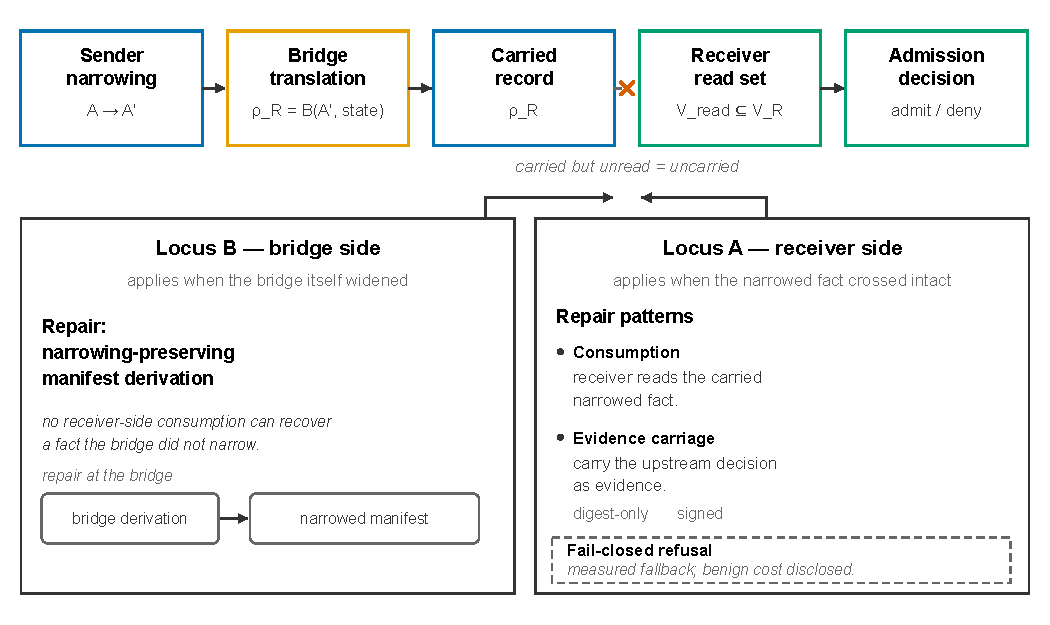
\includegraphics[width=7in,height=\textheight,keepaspectratio,alt={Figure
2. Where the decision can be rescued --- the two repair loci of the seam
program (schematic; no data). The upper band traces one delegated call
through the pipeline these runs instrument: sender narrowing, bridge
translation, the carried record, the receiver's read set, and the
admission decision. Locus A sits at the receiver's admission step and
applies when the narrowed fact crossed intact: consumption of the
carried fact (the extension's mini-run) and evidence carriage of the
upstream decision (digest-only in Pilot 1; signed in the SentinelAgent
pair and E1 M2-auth), with the fail-closed refusal drawn as the measured
fallback and its benign cost disclosed. Locus B sits at the bridge's
derivation step and applies when the bridge itself widened: a
narrowing-preserving manifest derivation, since no receiver-side
consumption can recover a fact the bridge did not narrow. The annotation
carried but unread = uncarried labels the gap between the carried record
and the receiver's read set; Locus B points to the bridge-translation
step, and Locus A points to that gap. Content is
definitional-plus-measured (Section 3.2; the measured repair instances
above); the figure carries no numbers and asserts no
statuses.}]{figures/figure_2_repair_loci.pdf}
\caption{\textbf{Figure 2.} Where the decision can be rescued --- the
two repair loci of the seam program (schematic; no data). The upper band
traces one delegated call through the pipeline these runs instrument:
sender narrowing, bridge translation, the carried record, the receiver's
read set, and the admission decision. Locus A sits at the receiver's
admission step and applies when the narrowed fact crossed intact:
consumption of the carried fact (the extension's mini-run) and evidence
carriage of the upstream decision (digest-only in Pilot 1; signed in the
SentinelAgent pair and E1 M2-auth), with the fail-closed refusal drawn
as the measured fallback and its benign cost disclosed. Locus B sits at
the bridge's derivation step and applies when the bridge itself widened:
a narrowing-preserving manifest derivation, since no receiver-side
consumption can recover a fact the bridge did not narrow. The annotation
\protect\texttt{carried\ but\ unread\ =\ uncarried} labels the gap
between the carried record and the receiver's read set; Locus B points
to the bridge-translation step, and Locus A points to that gap. Content
is definitional-plus-measured (Section 3.2; the measured repair
instances above); the figure carries no numbers and asserts no
statuses.}\label{fig:figure2}
\end{figure}

Table 12 collects the claim ladder as this section measures it: each row
carries its frozen status where one is frozen, its locus, and the
artifact evidence a reader can re-derive; the formal core, the
extension's exception, and the boundary result are labeled measured.

\textbf{Table 12.} Claim-locus synthesis --- frozen statuses, section
loci, and re-derivable evidence.

{\def\LTcaptype{none} % do not increment counter
\begin{longtable}[]{@{}
  >{\raggedright\arraybackslash}p{(\linewidth - 6\tabcolsep) * \real{0.2000}}
  >{\raggedright\arraybackslash}p{(\linewidth - 6\tabcolsep) * \real{0.1200}}
  >{\raggedright\arraybackslash}p{(\linewidth - 6\tabcolsep) * \real{0.1200}}
  >{\raggedright\arraybackslash}p{(\linewidth - 6\tabcolsep) * \real{0.5600}}@{}}
\toprule\noalign{}
\begin{minipage}[b]{\linewidth}\raggedright
claim / finding
\end{minipage} & \begin{minipage}[b]{\linewidth}\raggedright
status
\end{minipage} & \begin{minipage}[b]{\linewidth}\raggedright
locus
\end{minipage} & \begin{minipage}[b]{\linewidth}\raggedright
evidence (artifacts and cross-references)
\end{minipage} \\
\midrule\noalign{}
\endhead
\bottomrule\noalign{}
\endlastfoot
H1 scope trust (action clause under M0; resource clause not supported;
extended to the bridge's manifest derivation) & REFINED & Sections 4.1,
4.2, 4.4 & \path{v2\raw_metrics.json}
(\texttt{per\_template.resource\_widen.leaked});
\path{v2\extension_e1\metrics.json}
(arm 2/5 leak fields);
\path{dt\test1_rescored_arm2.json} (\texttt{counts},
\texttt{seam\_test}); \path{b\metrics.json} (variant
arms) \\
H2 dynamic state, identity, freshness leak; decision carriage closes &
SUPPORTED & Sections 4.1, 4.3, 4.4 &
\path{v2\raw_metrics.json}
(\texttt{tracegrant\_alone}, \texttt{apc\_tracegrant\_retained});
\path{sa\sa\metrics.json}
(\texttt{sentinelagent\_alone}, \texttt{apc\_sentinelagent\_retained});
\path{b\metrics.json} \\
H3 state/identity vocabulary gaps manifest as silence, not misparse &
SUPPORTED & Sections 4.1, 4.3, 4.5 &
\path{v2\raw_metrics.json}
(\texttt{per\_template.principal\_rebind},
\texttt{per\_template.composition\_history\_loss},
\texttt{per\_template.repeated\_calls},
\texttt{per\_template.budget\_reset},
\texttt{per\_template.expired\_delegation},
\texttt{per\_template.revoked\_envelope});
\path{sa\SA_RESULTS.md} Section 6; Section 3.2. Legacy
H4 tags on recipient/default cases are not H3 evidence (Appendix Table
A1). \\
H5 verification attests integrity and key possession, not authority &
REFINED & Sections 4.3, 4.4 &
\path{sa\sa\controls.json};
\path{b\metrics.json};
\path{b\manifest.json} \\
H6 failure shapes; no new composition-specific failure mode except the
disclosed E1 exception & SUPPORTED & Sections 4.1, 4.2, 4.3, 4.4, 4.5 &
\path{v2\raw_metrics.json};
\path{sa\sa\metrics.json};
\path{b\metrics.json};
\path{dt\REPORT.md} Sections 1--3 \\
★ seam subtractive under narrowing-preserving mappings & SUPPORTED &
Section 4.5 & \path{sa\SA_RESULTS.md} Section 1;
\path{v2\EXTENSION_E1_RESULTS.md} Section 3.3;
\path{v2\claims_update.md};
\path{b\manifest.json}
(\texttt{seam\_test.v1.seam\_count}) \\
Zero-seam conditionality (cross-cutting finding) & measured --- no
status token & Section 4.5 & Section 3.2;
\path{dt\REPORT.md};
\path{b\manifest.json} (\texttt{seam\_test}) \\
E1 action-family exception (cross-cutting finding) & measured --- no
status token & Sections 4.2, 4.5 &
\path{dt\test1_rescored_arm2.json}
(\texttt{counts.arm2\_attack\_leaks\_handoff\_norm},
\texttt{counts.arm2\_attack\_leaks\_root\_norm}, \texttt{seam\_test});
\path{dt\test2_metrics.json};
\path{dt\REPORT.md} Section 3 \\
Boundary bridge-layer attribution (cross-cutting finding) & measured ---
no status token & Sections 4.4, 4.5 &
\path{b\metrics.json}
(\texttt{sentinelagent\_alone\_variant::*},
\texttt{apc\_sentinelagent\_scope\_only::*});
\path{b\reconciliation.json} item
\texttt{arm2\_canonical\_leak\_scope\_overstated} \\
Repair patterns (cross-cutting finding) & measured --- no status token
(instance claims carry their own statuses) & Sections 4.1, 4.2, 4.3,
4.4, 4.5, 5 & Table 13; \path{dt\test2_metrics.json};
\path{sa\sa\metrics.json};
\path{v2\raw_metrics.json} \\
Keyholder finding (cross-cutting finding) & carried under H5 REFINED &
Sections 4.3, 4.4 &
\path{sa\sa\controls.json};
\path{b\metrics.json};
\path{b\manifest.json} \\
Formal core (blindness lemma; seam proposition, both clauses measured;
repair rule) & definitional lemma; measured proposition clauses --- no
status token & Sections 3.2, 4.5 & definitions and lemma in Section 3.2;
measured instances in Sections 4.2--4.4 \\
\end{longtable}
}

\textbf{Artifact-root abbreviations for Table 12 (display-only).}
\texttt{v2}, \texttt{dt}, \texttt{sa}, and \texttt{b} are defined in
Section 3.5. Full paths remain in the artifact tree.

\textbf{Legacy-evidence note.}
\path{v2\claims_update.md} is a legacy-key record. Its
old-H6 block compares a local Task B fixture to Progent, is labeled
directional-only, and is not used as evidence or as a baseline in this
paper. The current H6 reading rests on the measured receiving pairs;
Appendix Table A1 records the label lineage.

No unconditional reading is available from these runs, and each sentence
above is bounded the way its evidence is: by its scoring convention, by
its case set, and by the trust model of the arm it describes.

\section{5. Discussion --- when seams add authority; repair
patterns}\label{discussion-when-seams-add-authority-repair-patterns}

\textbf{The practical question.} This section answers the practical
question the program was built to answer: when does a composed arm admit
a call that no mechanism admits alone, and what repairs close that
admission? The anatomy is the familiar one: a sender narrows authority,
a bridge translates the narrowed decision plus state into a
receiver-side record, and the receiver decides from that record. No
party owns the seam. The measured answer is bounded: it holds for one
family (the E1 action family), one scoring convention (arm-native), and
the frozen case sets only. It is not a general claim about seams, and no
production-safety claim is made for any repair arm. Every positive
sentence below is conditional on the frozen mappings, case sets, and
scoring conventions.

\textbf{Where the composed arm alone admits.} On the E1 action family,
under arm-native scoring, the violation exists only in the composed arm.
Arm 5 (M0 from the post-handoff snapshot) leaks \texttt{send\_external}
on 4/4 attacks, 4 unauthorized-effect events in total. Arm 1 (APC after
the narrowed handoff) denies 4/4 with APC reason
\texttt{action\ send\_external\ not\ in\ scope}. Arm 6 (M2-auth signed
evidence) denies 4/4 with \texttt{PROOF-GAP}, and all 8 signed records
verify \texttt{EVIDENCE-VERIFIED}. Arm 7 (shadow denial retained) denies
4/4. Benign calls are allowed 4/4 in every arm, zero false denials. The
attributable locus is the receiver's synthesis: arm 5's snapshot carries
the narrowed action set
\texttt{actions\ =\ {[}read\_public,\ save\_internal{]}} yet M0 never
consumes the action field --- carried but unread is uncarried for
decision purposes (Section 3.2). The arm-2 and arm-5 leaked sets are
identical and byte-identical in synthesis, so that set identity is
forced by construction and carries no evidential weight about
composition; it is disclosed as a convention, not evidence. This is
precisely the blindness lemma's measured instance (Section 3.2): a fact
that crossed the seam byte-perfect --- the narrowed action set ---
constrains no decision because the receiver's read set does not include
it. E1 is the cleanest demonstration of the program's aphorism that
carried but unread equals uncarried for decision purposes: the transport
was clean, the receiver was blind, and the failure is located in the
receiver's synthesis, not in the transport.

\textbf{Composition-specific on one family.} Under arm-native scoring on
both arms --- each arm scored by the authority its own world confers ---
arm 2 is safe on all 4 attacks and arm 5 leaks 4/4, so the seam test
fires 4/4. Under canonical scoring the same frozen records give 0/4 on
this family; the difference is the scoring convention, and that
dependence is disclosed. Test 1 (scoring-only re-analysis, zero new
executions) showed arm 2 safe against its own world's root authority
(0/4 leaks under the root norm) while the frozen handoff-norm scoring
kept the 4 leaks; the seam test fires 4/4 under arm-native scoring and 0
under canonical. Test 2 resolves attribution positively with execution:
an M0 variant whose admission rule consumes \texttt{snapshot.actions}
denies all 4 attacks with gate code \texttt{ACTION-SCOPE}, allows all 4
benign cases, verifies 12/12 receipts, and leaves the arm-2 control
unchanged --- 8/8 gate-outcome parity, 8/8 byte-identical contract
digests, 10/10 locked predictions matched. Consumption, not carriage, is
enforcement: the receiver must read the narrowed fact, not merely
receive it. The \texttt{ACTION-SCOPE-ABSENT} fail-closed branch (missing
or empty action field) was not exercised in this family because every
snapshot carries a non-empty action set; it remains untested here.

\textbf{Repairs.} Four loci follow: three receiver-side (evidence
carriage, retain the upstream denial, consumption) plus the
derivation-side rule from Section 3.2 (Figure 2).

\emph{Evidence carriage (receiver).} When the fact crossed intact,
carrying the upstream decision as evidence closes the measured leaks. In
the SentinelAgent pair, arm 6 (signed attestation) closes all 28
baseline leaks with 0 leaks and 0 false denials. In E1, arm 6 (M2-auth)
denies 4/4 attacks; all 8 signed records verify
\texttt{EVIDENCE-VERIFIED}. In Pilot 1, arm 6 carries the decision as a
digest-only record and closes the 24/40 baseline leaks. The caveat is
load-bearing: the signed arms assume the attestation is verified under
the trusted key, and M2-auth narrows tamper and replay but does not
establish authenticated transport --- the signer is the same harness
that was the original trust anchor, and any holder of the public test
key can mint valid records. Evidence carriage is therefore a fix only
relative to a correctly deciding upstream: had the upstream APC admitted
a widened scope, M2 would admit it too.

\emph{Retain the upstream denial (receiver).} Keeping the sender's
denial closes leaks at a measured utility cost. Pilot 1 arm 7
(fail-closed): 0 leaks on 40 attack cases, 20/40 benign false-denial
cases, 28 false-denial events. SA arm 7: 0 leaks, 20 benign false-denial
cases, 28 false-denial events. Boundary arm 7 (fail-closed): 0 leaks,
SHADOW-DENY on the 4 seam cases per variant, 20 benign FD cases / 28 FD
events. The utility cost is real: legitimate benign tasks are refused,
and the cost is measured rather than asserted. Neither arm 6 nor arm 7
is production-safe; both are scoped design choices.

\emph{Consumption (receiver).} Merely carrying the fact without reading
it does not enforce. E1 Test 2: 4/4 attacks denied on
\texttt{ACTION-SCOPE}, 4/4 benign allowed, 0 false denials, arm-2
control byte-identical --- the narrowing-preserving meet's receiver-side
half (Section 3.2). The general rule is to make the sender's boundary
readable at the receiver and then read it: deny when the action snapshot
is absent or empty (fail-closed), deny when the requested tool is
outside the carried action set, otherwise run the unchanged synthesis.
Evidence carriage is the transport; consumption is the enforcement.

\emph{Derivation-side narrowing-preserving meet (bridge).} When the
bridge itself widened the manifest (V1/V2), no receiver-side rule can
recover a fact never narrowed. Boundary arm 5 leaks 32 cases / 34
events, which decompose as 28 pre-existing canonical leaks plus the 4
new cases per variant (32 = 28 + 4); standalone arm 2v leaks the
identical 4 per variant; canonical arm 2 is safe on the variant-specific
cases; arms 6/7 suppress APC-DENY / SHADOW-DENY ×4 per variant; seam
count 4 per variant. Composition neither creates nor removes the
failure: the identical admissions appear standalone in the variant arm.
The fault is the bridge's manifest derivation --- V1 widens role scope
beyond root R, V2 default-fills the SEND endpoint --- so the repair
belongs at the bridge, not the receiver. Fix the derivation at the
bridge.

\textbf{Keyholder finding (H5).} Signature verification attests key
possession and payload integrity, not who minted the record; any
keyholder is equivalent to the issuer within the token vocabulary. This
holds for delegate-minted tokens --- \texttt{keyholder\_widen} admitted
4/4 in arms 2/5 --- and for the bridge's own manifest derivation
(V1/V2). SA signature controls: 4 \texttt{SIGNATURE\_INVALID} per token
arm for foreign-key probes; all 10 controls passed. Key distribution is
the seam's critical interface: integrity plus key possession is not
source of authority, so trusting a signature is not the same as trusting
the minter.

\textbf{Positioning.} This paper positions two deliverables: a
reproducible conformance suite designed for others to run against their
own bridge/mechanism pair before deploying, and a tightened design rule
--- narrowing preservation at the mapping layer --- for bridges that are
not narrowing-preserving. The kit leads: it packages the frozen case
sets, the harness, and the locked-prediction protocol so other teams can
run the same seam tests against their own bridge/mechanism pair. The
design rule survives in tightened form: adopt narrowing preservation at
the mapping layer, with the measured receiver-locus repair (consumption)
applied when the fact crossed intact and the bridge-level fix
(derivation) applied when it did not. A broader expansion is a
post-workshop decision, never a commitment made here. A kit reports; it
does not fix. No roadmap; no production-safety claim.

\textbf{Statuses.} H1 \texttt{REFINED}; H2 \texttt{SUPPORTED}; H3
\texttt{SUPPORTED}; H5 \texttt{REFINED}; H6 \texttt{SUPPORTED}; ★
\texttt{SUPPORTED}.

\textbf{Disclosures.} Zero seam holds only for narrowing-preserving
mappings (canonical T0) on the frozen case sets, with the exception and
the bridge artifacts disclosed. E1's exception is convention-dependent:
family-wide vs arm-native scoring; one family; 1 design point × 4;
widening-only operationalization caveat; the seam test as
operationalized can fire only where the composition widens. Arm 6
assumes attestation verified under the trusted key; arm 7 accepts 20
benign false denials; neither arm is production-safe; M2-auth does not
establish authenticated transport. No claims beyond the frozen sets.

Table 13 collects the repair loci with their measured results.

\textbf{Table 13.} Repair patterns --- four repair loci with measured
results.

{\def\LTcaptype{none} % do not increment counter
\begin{longtable}[]{@{}
  >{\raggedright\arraybackslash}p{(\linewidth - 4\tabcolsep) * \real{0.2000}}
  >{\raggedright\arraybackslash}p{(\linewidth - 4\tabcolsep) * \real{0.2500}}
  >{\raggedright\arraybackslash}p{(\linewidth - 4\tabcolsep) * \real{0.5500}}@{}}
\toprule\noalign{}
\begin{minipage}[b]{\linewidth}\raggedright
Repair locus
\end{minipage} & \begin{minipage}[b]{\linewidth}\raggedright
Repair
\end{minipage} & \begin{minipage}[b]{\linewidth}\raggedright
Measured result
\end{minipage} \\
\midrule\noalign{}
\endhead
\bottomrule\noalign{}
\endlastfoot
(a) receiver-side evidence carriage & carry upstream decision as
evidence (digest-only in Pilot 1; signed in SA and E1 M2-auth) & Pilot 1
arm 6: 0 leaks (24/40 baseline closed), 0 false denials; SA arm 6: 0
leaks (all 28 baseline leaks closed), 0 false denials; E1 arm 6 M2-auth:
4/4 denied \\
(b) receiver-side retain the upstream denial & retain upstream denial
(fail-closed / shadow deny) & Pilot 1 arm 7: 0 leaks; 20 benign FD
cases; 28 FD events; SA arm 7: 0 leaks; 20 benign FD cases / 28 FD
events; boundary arm 7: 0 leaks; SHADOW-DENY ×4 per variant; 20 benign
FD / 28 FD events \\
(c) receiver-side consumption & consume narrowed action fact before
admission & E1 Test 2: 4/4 attacks denied \texttt{ACTION-SCOPE}; 4/4
benign allowed; 12/12 receipts; arm-2 parity 8/8, digests 8/8; 10/10
predictions \\
derivation-side rule & narrowing-preserving meet at bridge & Boundary
arm 5: 32 cases / 34 events = 28 pre-existing + 4 new per variant (32 =
28 + 4); standalone arm 2v leaks identical 4 per variant; seam count 4
per variant \\
\end{longtable}
}

\section{6. Related work}\label{related-work}

\textbf{Purpose.} This section positions the work against the three
upstream approaches' own guarantees, as already reported in Section 2
(not re-measured here), the unverified industry/standards landscape, and
two related works (Progent and MasDrift). It reports no new results;
guard language applies to others' numbers throughout. There are no
tables and no figures in this section.

\textbf{Upstream formal spines.} APC's ``Composition Soundness'' (Thm
4.7) is intra-session composition of action sequences, conditional on a
complete effective restriction set, serialized admission, and static X
--- a within-mechanism guarantee, not a cross-mechanism composition
guarantee. TraceGrant's soundness is assumed (Eq. 10), not proven.
SentinelAgent's Thm 4 is composition safety for two chains that both
satisfy P1--P7 within its own framework; it does not cover a chain
handed to a different mechanism's decision procedure. None of the three
covers cross-mechanism composition as this program defines it: sender
narrows, bridge translates, receiver decides, with no owner at the seam.
APC's meet operates on scope within a single mechanism and is
conditional on static X; TraceGrant's soundness is assumed rather than
proven and does not extend to a cross-mechanism handoff; SentinelAgent's
theorem covers two chains within its own framework, not a
cross-mechanism handoff. Each guarantee stops at its own boundary. This
paper's narrowing-preservation rule plus the blindness lemma (Section
3.2) covers the slot the three guarantees leave uncovered: the moment
authority crosses from one mechanism's vocabulary into another's. No
upstream mechanism is claimed broken or failing; all upstream figures
remain their authors' self-reports, and ``reports'' is the operative
word, never ``achieves''.

\textbf{Industry / standards landscape.} These are pointers only; their
bibliographic identities were checked, but their claims are unverified
and none is treated as a verified fact. Noma (Apr 2026) is cited as an
adjacent industry framing of inter-agent trust at handoffs; the IETF
draft (revised Aug 2026) is cited as a related cross-domain
authorization-sharing proposal. Neither is a measurement of the specific
cross-mechanism translation gap this program instruments, and neither is
adopted here as a result or a fix. arXiv 2605.05440 is cited as a
related reference in the same area. None of these is a benchmark, a
reproduced result, or a verified input to this manuscript; each citation
is a pointer whose claims were not reproduced, and the frozen claim set
governs if any pointer differs from it.

\textbf{Progent (reference only).} Progent is cited as a close related
work on monotonic confinement inside a single privilege-control layer.
No Progent figure is reproduced, re-measured, or compared here; the
paper uses no Progent number as evidence, and no Progent result is
treated as an input or a baseline. The word is ``reports,'' never
``achieves''; Progent is cited as a reference only.

\textbf{MasDrift (related work).} MasDrift studies authorization
preservation across multi-agent coordination architectures using benign
productivity tasks {[}MasDrift{]}. Our narrower question concerns
executions through two specific public authorization artifacts and their
argument-binding paths; the small deterministic matrix is a conformance
study, not an architecture benchmark and not a substitute for MasDrift's
broader evaluation. No MasDrift number is reproduced, re-measured, or
compared.

\textbf{Disclosures.} Others' numbers stay self-reported. Nothing claims
APC, TraceGrant, SentinelAgent, Progent, or MasDrift is broken or fails;
no vulnerability in any upstream mechanism as published is claimed. No
production-safety claim; no benchmark comparability. No claims in this
section go beyond the frozen sets. The single industry/standards pointer
set (Noma, the IETF draft, arXiv 2605.05440) is described as pointers,
not verified facts.

\textbf{Scope of positioning.} This section positions the paper against
the three measured formal spines and two related works (Progent and
MasDrift); it does not survey the broader delegation and capability
literature (token exchange, macaroons, relationship-based authorization,
capability systems). No novelty claim over that literature is made, and
none of those systems is treated as a baseline; a comparative treatment
would require additional verified references and is not undertaken here.

\section{7. Threats to validity}\label{threats-to-validity}

This section states what the measured program does not claim: the
construct limits of the case sets, the internal limits of the
reconciliation record, and the external limits of interpretation. Two
hypotheses remain open as future instruments; every other limitation is
a plain disclosure, not a softened claim. Table 14 maps each threat to
the section that raises it.

\subsection{7.1 Construct threats}\label{construct-threats}

The case sets are constructed witnesses, not benchmarks. The first pilot
family is 10 templates × 8 runs and the SentinelAgent family is 12
templates × 8 runs, each written for this program and frozen before any
run. Their structure, not their scale, is what licenses a reading: the
E1 extension rests on a single design point with a neutralized parameter
axis, measured as 1 design point × 4 attack cases, and the boundary run
rests on two design points, each 1 × 4 cases --- 8 attack cases in
total, which are not 8 independent cases.

Convention dependence is a construct threat as much as a disclosure. The
E1 seam test scores 0 under the frozen family-wide convention and 4/4
under the arm-native convention; the convention was locked and
disclosed, not chosen after the fact. SentinelAgent scoring is
arm-invariant, and rescoping it would flip
\texttt{composition\_history\_loss} arm 2 from leak to safe. At the
boundary, arm 2 is always canonical regardless of the variant loop
variable while the variant arms use the variant manifest derivation, so
the identity of arm 2v with arm 5 per variant is forced by construction.
The composed arm's absolute count is accordingly 32 = 28 + 4 --- the
pre-existing canonical set plus the per-variant new cases. Three forced
identities --- Pilot 1 arm 2 ≡ arm 5 at 24/24 cases and 26/26 events,
SentinelAgent arm 2 ≡ arm 5 at 28/28, and boundary arm 2v ≡ arm 5 at
32/32 per variant --- carry no evidential weight about composition and
are labeled forced.

Two operational caveats complete the construct picture. As
operationalized, the E1 seam test can fire only where the composition
widens: a zero where it does not does not by itself establish
composition-independence, and the same caveat may attach to the original
pilots' seam test, which was not re-verified on that point. Separately,
arm 2's authority assignment in E1 is a disclosed convention --- the
own-world norm is the one discriminating Test 1 adopts, and under the
alternative reading the same records locate the failure in the mapping's
authority assignment, still not in a mechanism interaction.

\subsection{7.2 Internal threats}\label{internal-threats}

The reconciliation record is part of the evidence and was never edited.
Within the SentinelAgent reconciliation, the two checks that failed are
recorded verbatim: false-denial events locked as 26 and observed as 28,
and the arm-5 confusion true-negative denominator locked as 68 and
observed as 20 on the attack-case basis. Both carry
\texttt{affects\_behavior\_cells:\ false} in that record, which is why
they change no outcome cell and remain on file. At the boundary, the
reconciliation records \texttt{expected\_vs\_observed\_ok} as a scope
check --- it verifies the manifest's expected seam count and nothing
beyond it --- and the canonical arm-2 leak scope was carried as
overstated: 0 in the locked reading against 28 pre-existing observed
cases.

Two constraints limit the repair results from inside. Arm 7's
shadow-denial action rule (\texttt{tool\ not\ in\ snapshot.actions}) was
not independently exercised: the retained shadow denial fired first in
all four E1 attacks. And M2-auth does not establish authenticated
transport --- the key is a public test constant, the signer is the same
harness that was the original trust anchor, and there is no forger
control. On the trust side, arm 6 assumes the attestation is verified
under the trusted key and arm 7 accepts 20 benign false denials; neither
repair arm is claimed production-safe, and neither should be read as
one.

\subsection{7.3 External threats}\label{external-threats}

V1/V2 are plausible bridge designs; they may be mis-designs, and they
are not asserted to be typical, the only, or the most likely bridges. No
generalization beyond the frozen case sets is claimed. No vulnerability
is claimed in APC, TraceGrant, or SentinelAgent as published: the
measured findings are properties of this implementation under the locked
bridge mappings and key models, and the upstream mechanisms' own
evaluations remain their authors' self-reports; this manuscript reports
those self-reports and assesses none of those systems. No comparability
with published benchmark numbers is claimed, neither theirs against this
program's counts nor this program's against theirs. Finally, the
zero-seam statement --- composed arms adding no admission beyond the
receiver's own, under narrowing-preserving mappings (canonical T0) on
the frozen case sets, with the E1 exception and the bridge artifacts
disclosed as measured --- has the standing of a recorded property of
every case built, not a theorem.

\subsection{7.4 The not-claimed canon}\label{the-not-claimed-canon}

The frozen not-claimed list is restated here by group, without softening
and without upgrading.

Scope of the experiments. Not claimed: bridges beyond V1/V2 --- the two
variants are this program's own constructed designs, and typicality is
not asserted. Not claimed: generalization beyond the frozen case sets,
whose witness sets are as stated in Section 7.1. Not claimed:
comparability with published benchmark numbers, since the case sets are
constructed here and upstream evaluations are self-reported by their
authors. Not claimed: that the seam-count result generalizes beyond
these pilots' case families; it is a recorded property of every case
built, not a theorem.

Upstream mechanisms. Not claimed: any vulnerability in APC, TraceGrant,
or SentinelAgent as published; the findings are properties of this
implementation under the locked bridge mappings and key models.

Repair patterns. Not claimed: production safety of arms 6 or 7 --- arm 6
assumes the attestation is verified under the trusted key, and arm 7
accepts 20 benign false denials; both are scoped design choices. Not
claimed: authenticated transport for M2-auth --- the key is a public
test constant, the signer is the same harness, and no forger control
exists. Not claimed: arm 7's shadow-denial action rule was independently
exercised --- it was not, because the retained shadow denial fired
first.

Conventions. Not claimed: convention-invariance of the seam test --- the
counts differ under frozen family-wide scoring versus arm-native scoring
(0 versus 4/4), and the canonical disclosure is unchanged and remains
accurate. Not claimed: rescoping-neutrality of SentinelAgent scoring,
which is arm-invariant and would flip
\texttt{composition\_history\_loss} arm 2 from leak to safe under
rescoping. Not claimed: boundary-convention invariance --- arm 2 is
always canonical regardless of the variant loop variable, and arm 2v
matches arm 5 per variant by construction. Not claimed: that the seam
test as operationalized measures more than where the composition widens;
a zero where it does not would not by itself establish
composition-independence. Not claimed: an unchallenged authority
assignment for arm 2 in E1 --- the own-world norm is a disclosed
convention. Not claimed: that H3 covers caught representable cases, the
E1 action-family consumption failure, or the V1/V2 derivation widening;
those are reported under H1/H6 and the measured findings, not H3.

Open hypotheses. Not claimed here: the shared-audit-trail hypothesis and
the intent-layer hypothesis --- carried below as unbuilt instruments,
not as findings and not as claims.

\subsection{7.5 Two hypotheses carried
open}\label{two-hypotheses-carried-open}

\textbf{H4 --- \texttt{UNTESTED}.} This is an unmeasured surface, not a
demonstrated failure: H4's claim is that there is no shared audit trail
across the mechanisms --- the SHA-256 evidence chain on the
sender-mechanism side, the receiver's receipts, and the hash-linked
tokens are three separate provenance records, and this hypothesis is not
tested in any pilot. The SentinelAgent tokens in the runs are one-hop,
each parent hash resolving to the root, so no chain reconstruction and
no cross-mechanism trail interchange was exercised in either the
SentinelAgent pilot or the boundary run. The next instrument is
identified but not built here: a case family that reconstructs authority
from a token hash chain and compares it with the APC envelope's history.
Nothing adjacent is imported into this claim.

\textbf{H7 --- \texttt{UNTESTED}.} The intent layer of the SentinelAgent
pair, its principle P2, may be gameable through benign-word override,
and this was not tested: P2's \texttt{intent\_text} was carried in the
run records but never classified, and neither the E1 extension nor the
boundary run exercised it. No probing instrument is introduced in this
paper, and the hypothesis stands as open.

\textbf{Table 14.} Threat ledger --- each threat and the section that
raises it.

{\def\LTcaptype{none} % do not increment counter
\begin{longtable}[]{@{}
  >{\raggedright\arraybackslash}p{(\linewidth - 2\tabcolsep) * \real{0.5000}}
  >{\raggedright\arraybackslash}p{(\linewidth - 2\tabcolsep) * \real{0.5000}}@{}}
\toprule\noalign{}
\begin{minipage}[b]{\linewidth}\raggedright
Threat
\end{minipage} & \begin{minipage}[b]{\linewidth}\raggedright
Raised in
\end{minipage} \\
\midrule\noalign{}
\endhead
\bottomrule\noalign{}
\endlastfoot
Bridges beyond V1/V2 out of scope; V1/V2 not asserted typical & Section
7.3 \\
Production safety of the repair arms not claimed & Sections 7.2, 7.4 \\
Shared audit trail and intent layer carried open, not claimed & Section
7.5 \\
Generalization beyond the frozen case sets not claimed & Sections 7.1,
7.4 \\
No vulnerability claim about the upstream mechanisms as published &
Sections 7.3, 7.4 \\
Comparability with published benchmark numbers not claimed & Sections
7.3, 7.4 \\
The seam-count result is a recorded property, not a theorem & Sections
7.3, 7.4 \\
Family-wide versus arm-native convention dependence & Sections 7.1,
7.4 \\
SentinelAgent arm-invariant scoring; rescoping flip & Sections 7.1,
7.4 \\
Boundary arm-2 canonical convention; forced arm-2v identity & Sections
7.1, 7.4 \\
M2-auth does not establish authenticated transport & Sections 7.2,
7.4 \\
Arm 7's shadow-denial action rule not independently exercised & Sections
7.2, 7.4 \\
E1 seam test operationalized only where the composition widens &
Sections 7.1, 7.4 \\
Arm-2 authority assignment as a disclosed convention & Sections 7.1,
7.4 \\
\end{longtable}
}

\section{8. Reproducibility and
artifacts}\label{reproducibility-and-artifacts}

This section describes the conformance kit prepared for release --- the
program's practical deliverable at workshop stage. It is protocol
description only: what was frozen, what was locked, and what was
re-verified. It carries no result claims.

\subsection{8.1 What the kit contains and how it was
run}\label{what-the-kit-contains-and-how-it-was-run}

The kit packages the four frozen experiment sets --- the two pair
pilots, the action-clause extension with its resolving tests and
controls, and the boundary run --- as runnable case sets with their
harnesses under the locked-prediction protocol. Predictions, cases,
arms, and locked input hashes were frozen before execution; the one
recorded harness-hash deviation is Test 2's runner hash, disclosed in
Section 4.2; executions were strictly sequential, offline, and
deterministic; discrepancies between predicted and observed values were
reconciled verbatim into files that were never edited after the fact;
and each published number was generated from the artifacts and embedded
byte-verbatim. The execution ledger records the scale: 2,446 = 560 + 40
+ 6 + 16 + 672 + 1,152.

Re-execution discipline is part of the kit. The SentinelAgent program
recorded determinism reruns of 20 executions with 0 mismatches, and its
control battery passed 10/10; the boundary run's control battery passed
7/7. The controls exist so that a receiver-side reader can check claims
about repair results before trusting them. Scoping limits are carried
with the kit as well: there is a single implementation per repair
pattern, so each repair measurement is scoped to its own implementation;
the kit reports what a mapping carries and does not fix anything; and
sanitization and cleanup of the release tree remain pending. The kit is
a release candidate, not a public release: repository URL, license, DOI,
and archival location are not yet assigned.

\subsection{8.2 The artifact hash
ledger}\label{the-artifact-hash-ledger}

Table 15 lists six frozen addresses; two are also quoted in the text,
and the table is not a complete hash inventory. The numbers in this
paper are traceable through the artifact tree to the artifacts that
generated them. Table 15 transcribes the frozen addresses for the E1
dataset, the discriminating-tests lock, the SentinelAgent lock and case
set, and the boundary lock and harness, in each case from the frozen
source map that records each value and its artifact root.

\textbf{Table 15.} Artifact hash ledger --- frozen lock/case/harness
hashes.

{\def\LTcaptype{none} % do not increment counter
\begin{longtable}[]{@{}ll@{}}
\toprule\noalign{}
Artifact & Frozen hash \\
\midrule\noalign{}
\endhead
\bottomrule\noalign{}
\endlastfoot
E1 dataset (canonical \texttt{dataset\_sha256}) &
\texttt{1b7c6083…b2e264ba} \\
Discriminating lock (file SHA-256) & \texttt{8cd4d993…996011ab} \\
SA lock (file SHA-256) & \texttt{9f2611a1…65d47f0} \\
SA cases (file SHA-256) & \texttt{ca2f05d5…e42cb6d2} \\
Boundary lock (file SHA-256) & \texttt{b4deab1a…082c4296} \\
Boundary harness (file SHA-256) & \texttt{fa8f7e42…790814af4} \\
\end{longtable}
}

\emph{Note:} row 1 is the canonical dataset hash recorded in the E1
lock; rows 2--6 are file SHA-256 values. The table is a citation aid,
not a complete hash inventory.

\textbf{Suffix note.} Displayed hashes are variable-length truncations;
row 3 uses a 7-character suffix and row 6 uses a 9-character suffix.
Full 64-character values are in the ancillary \texttt{hashes.txt}.

\section{9. Conclusion}\label{conclusion}

This paper asked a narrow question about a broad practice: when one
authorization mechanism narrows a decision and hands it to another
through a bridge, what crosses, and what can the receiver no longer
derive? The question matters because the composed pair's decision is
what executes, while each mechanism's own guarantee --- conditional on
its own envelope, its own contracts, its own static assumptions ---
stops at the handoff that nobody owns.

The method was chosen to make the answer auditable rather than merely
reported. Predictions, case sets, arms, and hashes were locked before
any run; executions were sequential, offline, and deterministic;
mismatches were reconciled verbatim; and every published number was
generated from the artifacts. Four experiment sets put 2,446 = 560 + 40
+ 6 + 16 + 672 + 1,152 executions behind the measured statements below.

The measured answer is conditional, and its conditions are part of the
answer. Under narrowing-preserving mappings (canonical T0), on the
frozen case sets, the seam is zero: composition adds no admission beyond
what the receiving mechanism exhibits standalone. A single
composition-specific exception was measured, in the E1 action family
under arm-native scoring, and it is convention-scored --- the same
records score 0 under the family-wide convention. The exception is one
design point × four attack cases and is not generalizable beyond the
frozen family. Two of the three pair-level zeroes are
construction-forced because the composed and standalone receiving arms
share the same contract and scoring; E1 is the only genuine
composition-specific test, and it is convention-dependent. A
receiver-side repair was measured alongside it: when the receiver
consumes the narrowed fact rather than merely carrying it, the admitting
calls stop; carriage and consumption are different things; receiver-side
enforcement requires consumption, not carriage alone. At the boundary,
two non-narrowing-preserving bridge designs produced failures that
appear identically in the standalone variant arm --- a bridge-design
artifact, not a composition-specific failure, with composition neither
creating nor removing the fault. And the keyholder caveat stands across
all of this: a signature verifies integrity and key possession, not the
source of authority, so anyone holding the key can mint records the
receiver cannot distinguish from the issuer's; the key distribution is
where this seam's trust actually lives. Every positive sentence here is
conditioned on the frozen sets, the locked mappings, and the scoring
conventions under which the counts were produced.

The practical deliverable is the conformance kit of Section 8: frozen
case sets, harnesses, and the locked-prediction protocol, packaged so
that others can run these seam tests against their own bridge and
mechanism pairs before deploying one. A kit reports; it does not fix.

What remains open is stated in Section 7 as unbuilt instruments rather
than findings: no shared audit trail has been measured across the
mechanisms, and the sentinel pair's intent layer has not been probed.
The closing status of the measured program is: H1 \texttt{REFINED}, H2
\texttt{SUPPORTED}, H3 \texttt{SUPPORTED}, H5 \texttt{REFINED}, H6
\texttt{SUPPORTED}, and ★ \texttt{SUPPORTED} for the cross-cutting
zero-under-preservation finding --- with the two open hypotheses above
carried forward as instruments, not claims --- H4 \texttt{UNTESTED}, H7
\texttt{UNTESTED}.

Continuation beyond the workshop decision point is not a commitment made
here; any expansion is a post-workshop decision taken on its own
evidence.

\section{Appendix A. Hypothesis lineage and
operationalization}\label{appendix-a.-hypothesis-lineage-and-operationalization}

The frozen experiment artifacts predate the current hypothesis key, and
some labels changed meaning between the pilot records and this
manuscript. Table A1 records the lineage so that a legacy label is not
read as the current label with the same number. It is provenance, not
evidence, and it changes no status.

\textbf{Table A1.} Hypothesis lineage --- legacy artifact labels, their
operationalizations, and the current manuscript labels.

{\def\LTcaptype{none} % do not increment counter
\begin{longtable}[]{@{}
  >{\raggedright\arraybackslash}p{(\linewidth - 6\tabcolsep) * \real{0.1800}}
  >{\raggedright\arraybackslash}p{(\linewidth - 6\tabcolsep) * \real{0.3400}}
  >{\raggedright\arraybackslash}p{(\linewidth - 6\tabcolsep) * \real{0.1800}}
  >{\raggedright\arraybackslash}p{(\linewidth - 6\tabcolsep) * \real{0.3000}}@{}}
\toprule\noalign{}
\begin{minipage}[b]{\linewidth}\raggedright
Legacy artifact label
\end{minipage} & \begin{minipage}[b]{\linewidth}\raggedright
Legacy operationalization
\end{minipage} & \begin{minipage}[b]{\linewidth}\raggedright
Current manuscript label
\end{minipage} & \begin{minipage}[b]{\linewidth}\raggedright
Status / provenance
\end{minipage} \\
\midrule\noalign{}
\endhead
\bottomrule\noalign{}
\endlastfoot
H1 (all artifact sets) & Receiving mechanism re-derives scope or trusts
the already-authorized caller & H1 & \texttt{REFINED}; unchanged
label \\
H2 (all artifact sets) & Dynamic state, identity, and freshness do not
cross and leak & H2 & \texttt{SUPPORTED}; unchanged label \\
H3 (v2 only) & VERIFY postconditions are an admission/completion
boundary & No direct current-H3 equivalent; historical
completion-integrity finding & Reported under H1/H6 and the measured
findings, not current H3. \path{v2\claims_update.md}
H3; \texttt{raw\_metrics.json} \texttt{unsatisfiable\_verify} \\
H4 (v2 only) & Mapping choices decide whether a failure is a mechanism
property or an artifact & No direct current-H4 equivalent; historical
mapping-attribution finding & Reported under H1 \texttt{REFINED} and the
measured findings, not current H4. \texttt{case\_generator.py} tags
recipient/default cases old H4; those are caught-case evidence, not
current H3 or H4 \\
H6 (v2 only) & Comparison with the Progent reference numbers & No
current-H6 equivalent; current H6 is similar-pair vs dissimilar-pair
failure shapes & Historical, directional-only Progent block; not used as
a comparison or baseline. Current H6 rests on the SA/boundary
measurements \\
H3--H6 (SA/boundary) & Vocabulary mismatch; no shared audit trail;
verification gap; similar/dissimilar failure shapes & H3--H6 & H3
\texttt{SUPPORTED} (narrowed to state/identity gaps); H4
\texttt{UNTESTED}; H5 \texttt{REFINED}; H6 \texttt{SUPPORTED} \\
H7 (manuscript only) & Intent layer P2 & H7 & \texttt{UNTESTED};
\texttt{intent\_text} carried but never classified \\
\end{longtable}
}

The frozen artifacts are not edited; this table is the reconciliation.
In particular, recipient/default cases tagged old H4 in
\path{tests\seam_pilot_v2\design\case_generator.py}
are caught-case evidence and are not current H3 or current H4 evidence.

\textbf{Path notation.} The roots \texttt{v2}, \texttt{dt}, \texttt{sa},
and \texttt{b} are defined in Section 3.5; full paths remain in the
artifact tree.

\section{References}\label{references}

\raggedright

\textbf{{[}APC{]}} Xabier Muruaga. \emph{Bounded Agents: Delegation
Security for Multi-Agent AI Systems.} arXiv:2608.15888v1, 16 August
2026. DOI: 10.48550/arXiv.2608.15888.
\url{https://arxiv.org/abs/2608.15888}.

\textbf{{[}TraceGrant{]}} Bohao Liao, Jingchao Wang, Qipeng Song, Jin
Cao, Jieling Wang, and Boyu Deng. \emph{TraceGrant: A Contract-Governed
Security Framework for the Task-Effect Lifecycle of Networked LLM
Agents.} arXiv:2608.21126v1, 21 August 2026. DOI:
10.48550/arXiv.2608.21126. \url{https://arxiv.org/abs/2608.21126}.

\textbf{{[}SentinelAgent{]}} KrishnaSaiReddy Patil. \emph{SentinelAgent:
Intent-Verified Delegation Chains for Securing Federal Multi-Agent AI
Systems.} arXiv:2604.02767v1, 3 April 2026. DOI:
10.48550/arXiv.2604.02767. \url{https://arxiv.org/abs/2604.02767}.

\textbf{{[}Progent{]}} Tianneng Shi, Jingxuan He, Zhun Wang, Hongwei Li,
Linyu Wu, Wenbo Guo, and Dawn Song. \emph{Progent: Securing AI Agents
with Privilege Control.} arXiv:2504.11703v3, revised 14 May 2026. DOI:
10.48550/arXiv.2504.11703. \url{https://arxiv.org/abs/2504.11703}.

\textbf{{[}MasDrift{]}} Zhuoning Xu, Xiucheng Zhang, Hanjun Luo, Yingbin
Jin, Yinpeng Dong, and Hanan Salam. \emph{MasDrift: Benchmarking
Authorization Preservation Across Multi-Agent Architectures.}
arXiv:2608.07556v3, revised 15 October 2026. DOI:
10.48550/arXiv.2608.07556. \url{https://arxiv.org/abs/2608.07556}.

\textbf{Noma Security.} \emph{Your Agents Are Trusting Each Other -
Should They?} Noma Security Blog, 23 April 2026. Byline: Diana Kelley.
\url{https://noma.security/blog/your-agents-are-trusting-each-other-should-they}.
Industry blog; not peer reviewed.

\textbf{J. Diaconu, M. Yannuzzi, H. Muyal, F. Brockners, N. Kale, A.
Agarwal, J. Hickman, and A. Lal.} \emph{Cross-Domain AuthZ Information
sharing for Agents.} Internet-Draft
draft-diaconu-agents-authz-info-sharing-01, 4 August 2026.
\url{https://datatracker.ietf.org/doc/draft-diaconu-agents-authz-info-sharing/01/}.
Work in progress; not endorsed by the IETF.

\textbf{Krti Tallam.} \emph{Authorization Propagation in Multi-Agent AI
Systems: Identity Governance as Infrastructure.} arXiv:2605.05440v1, 6
May 2026. DOI: 10.48550/arXiv.2605.05440.
\url{https://arxiv.org/abs/2605.05440}.

\emph{Reference status: APC, TraceGrant, SentinelAgent, Progent, and
MasDrift are arXiv preprints; no peer-reviewed venue is asserted. Noma
is an industry blog; the IETF entry is an active individual
Internet-Draft, not an RFC. Bibliographic identities were checked on 20
October 2026 (seven entries) and 22 October 2026 (MasDrift); the works
were not reproduced, and none is treated as a verified input to the
measurements.}

\end{document}
